%%%%%%%%%%%%%%%%%%%%%%%%%%%%%%%%%%%%%%%%%%%%%%%%%%%
%% LaTeX  book                                   %%
%% Author:                                       %%
%% License:                                      %%
%%%%%%%%%%%%%%%%%%%%%%%%%%%%%%%%%%%%%%%%%%%%%%%%%%%
\documentclass[12pt]{book}
\usepackage{iftex}
\ifPDFTeX
  % PDFLaTeX or LaTeX 
  \usepackage[utf8]{inputenc}
  \usepackage[T1]{fontenc}
  \DeclareUnicodeCharacter{00B5}{\ensuremath{\mu}}
\else
  %  XeLaTeX or LuaLaTeX
  \usepackage{fontspec}
\fi
\usepackage[left=2cm,right=1cm,top=2cm,bottom=2cm,headheight=1cm]{geometry}
\usepackage{lmodern}
\usepackage{amsmath}

\usepackage{textcomp}
\usepackage{multicol}
\usepackage[]{ragged2e}
\usepackage[dvipsnames]{xcolor}
\usepackage{blindtext}
%%%%%
\usepackage[12pt]{moresize}
%\fontsize{8}{20}\selectfont
\usepackage{amssymb}
\usepackage{enumerate}
\usepackage{graphicx}
\usepackage{gensymb}
%%%%%
\usepackage{pifont}
\usepackage{braket}
\usepackage{esint}
\usepackage{ziffer}
\usepackage{latexsym}
\usepackage[normalem]{ulem}
\usepackage{color,tikz}
\usepackage{mathtools}
\usepackage{setspace}
\usepackage{tocloft}
\usepackage{longtable}
\usepackage{url}
\usepackage{booktabs}
\usepackage{float}
\usepackage{graphicx, nicefrac}
\usepackage{scalefnt}
\usepackage{tikz}
\usepackage[sans]{dsfont}
\usetikzlibrary{decorations.pathmorphing}
\usetikzlibrary{shapes.geometric, arrows}
\usepackage[ruled, vlined, linesnumbered]{algorithm}
\usepackage{caption}%
\usepackage[Sonny]{fncychap}
\usepackage[weather, clock]{ifsym}
\usepackage[most]{tcolorbox}
\usepackage{MnSymbol}
%%%%%%%%%%%%%%%%%%%%%%%%%%%%%%%%%%%%%%%%%%%%%%%%%%%%%%%%%
% Configurações para o Maxima %
%%%%%%%%%%%%%%%%%%%%%%%%%%%%%%%%%%%%%%%%%%%%%%%%%%%%%%%%%
\usepackage{upgreek}
\usepackage{xcolor}
\usepackage{longtable,booktabs,array}
\usepackage{calc} % for calculating minipage widths
% Correct order of tables after \paragraph or \subparagraph
\usepackage{etoolbox}
\usepackage{grffile}
\usepackage{ifthen}
\newsavebox{\picturebox}
\newlength{\pictureboxwidth}
\newlength{\pictureboxheight}
\newcommand{\includeimage}[1]{
    \savebox{\picturebox}{\includegraphics{#1}}
    \settoheight{\pictureboxheight}{\usebox{\picturebox}}
    \settowidth{\pictureboxwidth}{\usebox{\picturebox}}
    \ifthenelse{\lengthtest{\pictureboxwidth > .95\linewidth}}
    {
        \includegraphics[width=.95\linewidth,height=.80\textheight,keepaspectratio]{#1}
    }
    {
        \ifthenelse{\lengthtest{\pictureboxheight>.80\textheight}}
        {
            \includegraphics[width=.95\linewidth,height=.80\textheight,keepaspectratio]{#1}
            
        }
        {
            \includegraphics{#1}
        }
    }
}
\newlength{\thislabelwidth}
\DeclareMathOperator{\abs}{abs}

\definecolor{labelcolor}{RGB}{100,0,0}
\usepackage{physics}
%%%%%%%%%%%%%%%%%%%%%%%%%%%%%%%%%%%%%%%%%%%%%%%%%%%%%%%%%
% Source: http://en.wikibooks.org/wiki/LaTeX/Hyperlinks %
%%%%%%%%%%%%%%%%%%%%%%%%%%%%%%%%%%%%%%%%%%%%%%%%%%%%%%%%%
\usepackage{hyperref}
%\usepackage{graphicx}
\usepackage[portuguese]{babel}

%%%%%%%%%%%%%%%%%%%%%%%%%%%%%%%%%%%%%%%%%%%%%%%%%%%%%%%%%%%%%%%%%%%%%%%%%%%%%%%%
% 'dedication' environment: To add a dedication paragraph at the start of book %
% Source: http://www.tug.org/pipermail/texhax/2010-June/015184.html            %
%%%%%%%%%%%%%%%%%%%%%%%%%%%%%%%%%%%%%%%%%%%%%%%%%%%%%%%%%%%%%%%%%%%%%%%%%%%%%%%%
\newenvironment{dedication}
{
   \cleardoublepage
   \thispagestyle{empty}
   \vspace*{\stretch{1}}
   \hfill
   \begin{minipage}[t]{0.66\textwidth}
   \raggedright
}
{
   \end{minipage}
   \vspace*{\stretch{3}}
   \clearpage
}

%%%%%%%%%%%%%%%%%%%%%%%%%%%%%%%%%%%%%%%%%%%%%%%%
% Chapter quote at the start of chapter        %
% Source: http://tex.stackexchange.com/a/53380 %
%%%%%%%%%%%%%%%%%%%%%%%%%%%%%%%%%%%%%%%%%%%%%%%%
\makeatletter
\renewcommand{\@chapapp}{}% Not necessary...
\newenvironment{chapquote}[2][2em]
  {\setlength{\@tempdima}{#1}%
   \def\chapquote@author{#2}%
   \parshape 1 \@tempdima \dimexpr\textwidth-2\@tempdima\relax%
   \itshape}
  {\par\normalfont\hfill--\ \chapquote@author\hspace*{\@tempdima}\par\bigskip}
\makeatother

%%%%%%%%%%%%%%%%%%%%%%%%%%%%%%%%%%%%%%%%%%%%%%%%%%%
% First page of book which contains 'stuff' like: %
%  - Book title, subtitle                         %
%  - Book author name                             %
%%%%%%%%%%%%%%%%%%%%%%%%%%%%%%%%%%%%%%%%%%%%%%%%%%%

% Book's title and subtitle
\title{\Huge \textbf{\MakeUppercase{Simulações de Ondulatória com Uso do Maxima}} \footnote{This is a footnote.} \\  }
% Author
\author{\textsc{Elielzer Nuayed}\thanks{\url{https://github.com/elielzer}}}


\begin{document}
\frontmatter
\maketitle

%%%%%%%%%%%%%%%%%%%%%%%%%%%%%%%%%%%%%%%%%%%%%%%%%%%%%%%%%%%%%%%
% Add a dedication paragraph to dedicate your book to someone %
%%%%%%%%%%%%%%%%%%%%%%%%%%%%%%%%%%%%%%%%%%%%%%%%%%%%%%%%%%%%%%%
\begin{dedication}
Dedicated to Calvin and Hobbes.
\end{dedication}

%%%%%%%%%%%%%%%%%%%%%%%%%%%%%%%%%%%%%%%%%%%%%%%%%%%%%%%%%%%%%%%%%%%%%%%%
% Auto-generated table of contents, list of figures and list of tables %
%%%%%%%%%%%%%%%%%%%%%%%%%%%%%%%%%%%%%%%%%%%%%%%%%%%%%%%%%%%%%%%%%%%%%%%%
{\tableofcontents}
%{\listoffigures}
%{\listoftables}

\mainmatter

%%%%%%%%%%%
% Prefácio%
%%%%%%%%%%%
\chapter*{Prefácio}
Este livro foi concebido a partir de um \emph{insight} pessoal após eu ler um anúncio sobre uso do \emph{Maxima} no ensino da Física. Então veio-me a ideia de escrever algo nesse sentido.
Escolhi sobre ondulatória. O Maxima é introduzido no contexto como ambiente de apoio no momento que seja necessário simular as proposições. Dentre as proposições abordaremos situações clássicas, pois o objetivo é justamente apresentar o cartel de ferramentas desse software adequadas para transcrever a linguagem da física para representar as situações problema.

É provável que o leitor se defronte aqui com uma versão do wxMaxima diferente daquele que esteja instalada em seu computador, porém isso deve não impactar no entendimento do que é exposto no livro, pois o núcleo principal do Maxima mantém-se inalterado quanto a sua finalidade.

%%%%%%%%%%%%%%%%
% INTRODUÇÃO   %
%%%%%%%%%%%%%%%%
\chapter{INTRODUÇÃO}
\section{Sobre o Maxima}
De acordo com descrição no site fabricante, o Maxima é um programa de computador do tipo multiplataforma, ou seja, ele está preparado para trabalhar (compilar) sob diversos sistemas operacionais ou plataformas computacionais.
Ainda de acordo com esse site o Maxima é uma versão evoluída de software especialista Macsyma. Os sistemas especialistas foram criados com a finalidade de reproduzir o raciocínio ou expertise de um  profissional de alguma área de conhecimento específica.

Assim,o Maxima é um sistema especialista para a manipulação de expressões matemáticas, tanto na forma simbólica como na forma numérica, incluindo:
\begin{itemize}
	\item diferenciação,
	\item integração,
	\item séries de Taylor,
	\item transformadas de Laplace,
	\item equações diferenciais ordinárias,
	\item sistemas de equações lineares,
	\item polinômios,
	\item conjuntos,
	\item listas,
	\item vetores,
	\item matrizes e
	\item tensores.
\end{itemize}

\noindent O que caracteriza a matemática simbólica é de não estar atrelada a um determinado idioma, por exemplo a expressão algébrica: \(x+2=7\), tem o mesmo significado em qualquer idioma. Portanto o Maxima é um sistema algébrico computacional para auxílio no cálculo e manipulação da  matemática simbólica visado simplificar o esforço de trabalho do estudante ou profissional (professor ou pesquisador).

O Maxima produz também resultados numéricos de alta precisão usando frações exatas, inteiros de precisão arbitrária e números de ponto flutuante de precisão variável. O Maxima pode plotar funções e dados em duas e três dimensões. Utilizaremos em nossos desenvolvimentos a plataforma gráfica do wxMaxima\textregistered .


\section{Trabalhando com o wxMaxima}
O Maxima é constituído de \emph{packages} (pacotes). Um pacote vem corresponder a uma biblioteca de comandos programados para uma finalidade específica, e pode ser carregado para o ambiente por meio do comando \emph{load}, alguns pacotes são carregados automaticamente ao abrir o WMaxima.

Cada pacote possui uma chave específica que é usada como argumento do comando \emph{load} Exemplos:
\begin{itemize}
	\item load(physical\_constants){\$} 
	\item load(worldmap){\$}
	\item load(unit){\$}
\end{itemize}
Experimente testar o comando \emph{load}, como no exemplo a seguir:
\begin{figure}[H]
	\centering
	\caption{Exemplo de como invocar um pacote para o ambiente do Maxima}
	\label{fig:mnewton}
	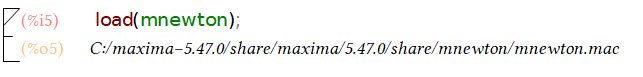
\includegraphics[width=1\linewidth]{mnewton}
\end{figure}


A base de conhecimento do Maxima, de acordo com sua documentação, é organizada por meio de um conjunto de categorias, por exemplo: Expressões, Operadores, Avaliação de Expressões, Simplificação, Plotagem, etc.

Há dois tipos de comandos específicos: as \emph{tags} (ou variáveis de controle) e as funções. 
Algumas funções possuem o mesmo nome das tags. Geralmente as tags servem para comutar dois estados ,o \emph{true} ou \emph{false}, um desses será o valor padrão (\emph{default}).

Vamos tomar como primeiro exemplo a fórmula do teorema de Pitágoras. Vamos escrever no \emph{prompt} do wxMaxima a seguinte expressão: \textsf{c\^\ 2+b\^\ 2=a\^\ 2}
\begin{figure}[H]
	\centering
	\caption{Entrando uma expressão algébrica.}
	\label{fig:pitagoras}
	%\begin{Center}
	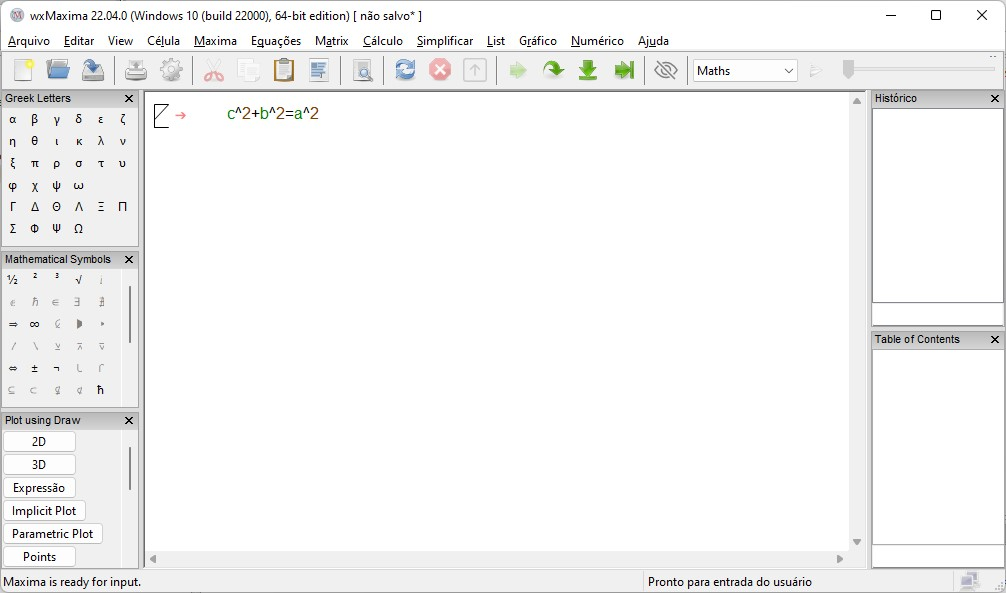
\includegraphics[scale=0.5]{pitagoras.jpg}
	%\end{Center}
\end{figure}

\noindent Essa expressão é o input do processo. O Maxima processará essa entrada após acionada a combinação de tecla \texttt{Shift+Enter} do que, em seguida, apresentará uma saída na área do \emph{prompt}, figura \ref{fig:pitagoras-2}.

\begin{figure}[ht]
	\centering
	\caption{Saída apresentada após após processamento da expressão algébrica entrada.}
	\label{fig:pitagoras-2}
	%\begin{Center}
	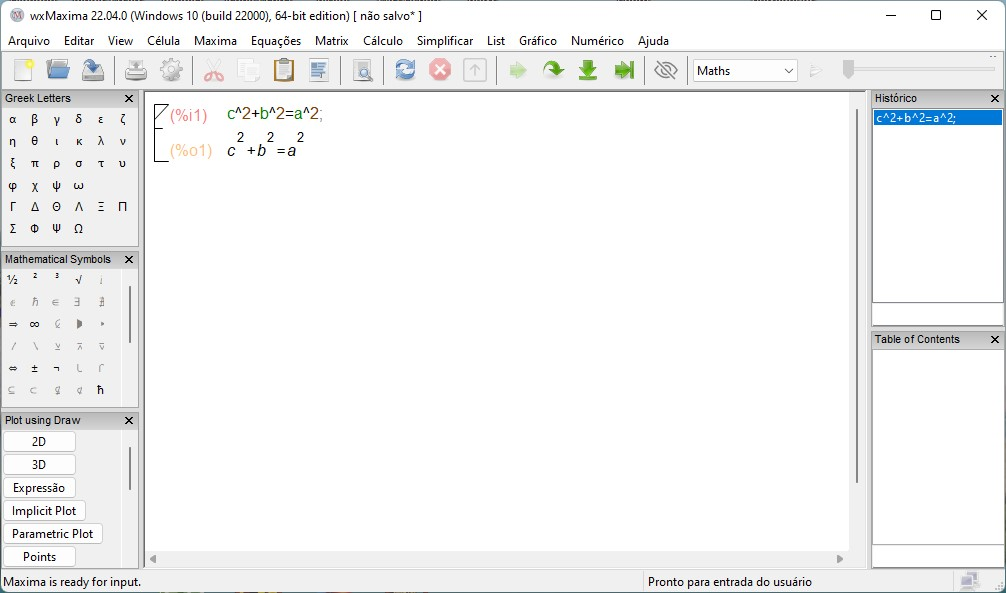
\includegraphics[scale=0.5]{pitagoras-2.jpg}
	%\end{Center}
\end{figure}
\pagebreak
\noindent Observe que o resultado é disponibilizado com identificadores chamados \texttt{label}, tais que:

\begin{minipage}[]{4.000000em}\color{red}\bfseries (\% i1)	
\end{minipage}é o \emph{label} indica a entrada ou \emph{input}, e 

%%%%

\begin{minipage}[]{4.000000em}\color{green}\bfseries (\% o1)	
\end{minipage}é o \emph{label} que indica a saída ou \emph{output}.


No Maxima é possível \emph{nomear uma expressão} de forma que possa ser reutilizada. Por exemplo, escrevendo no prompt a seguinte expressão: \textsf{pitg:c\^\ 2+b\^\ 2=a\^\ 2}. Observe o resultado disso na figura \ref{fig:pitagoras-3}.
\begin{figure}[ht]
	\centering
	\caption{Nomeando expressões.}
	\label{fig:pitagoras-3}
	%\begin{Center}
	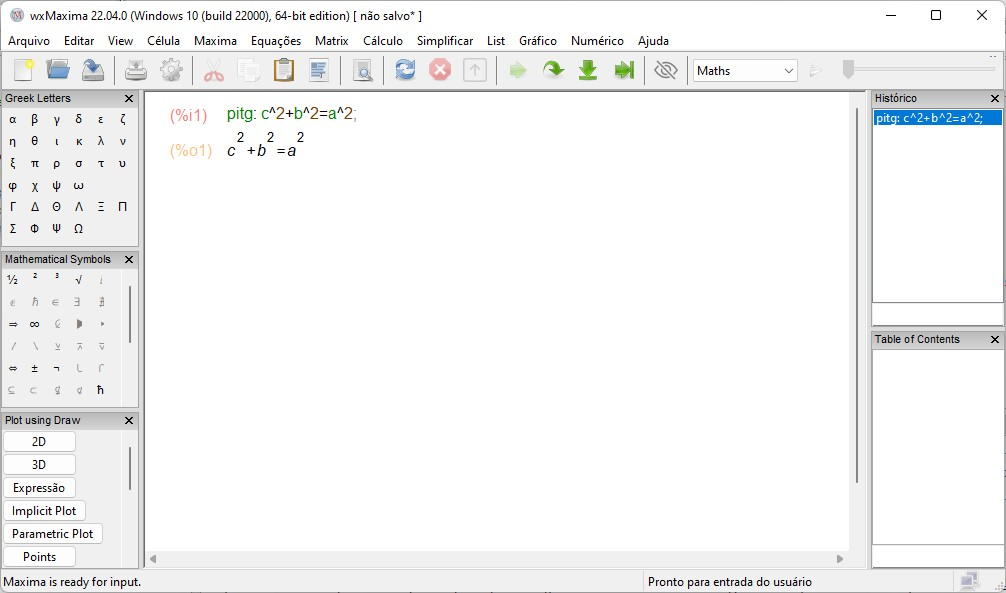
\includegraphics[scale=0.5]{pitagoras-3.jpg}
	%\end{Center}
\end{figure}


\noindent Essa ação de nomear as expressões algébricas é importante pois facilita a reutilização recorrente da fórmula. Por exemplo, com a seguinte expressão nomeada \textsf{sol1:solve(pitg,a)}. O termo \emph{solve} corresponde a uma fórmula (função) interna do Maxima. Os resultados aparecem na figura \ref{fig:pitagoras-4}. 
\begin{figure}[ht!]
	\centering
	\caption{Usando expressões.}
	\label{fig:pitagoras-4}
	%\begin{Center}
	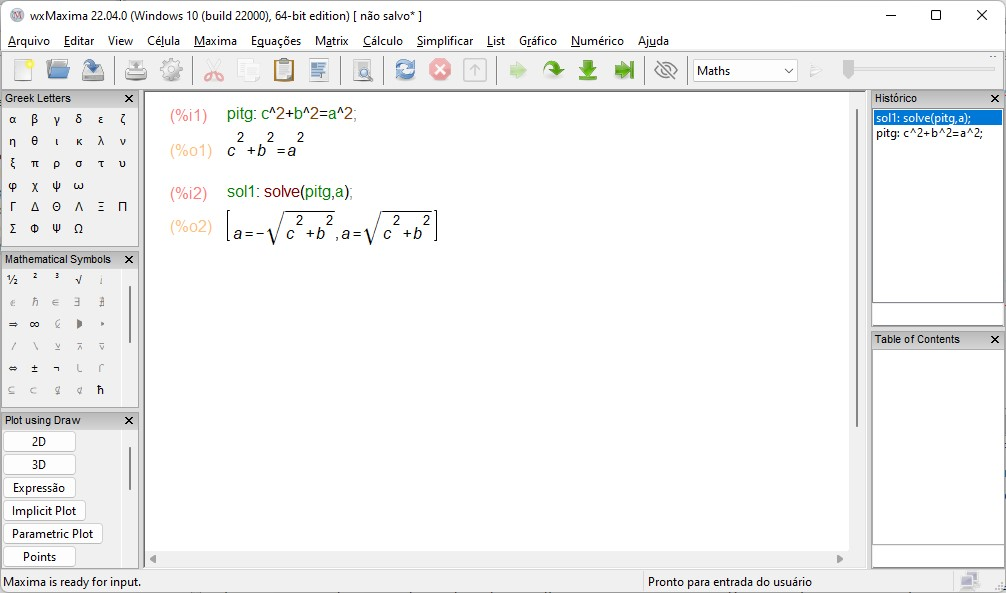
\includegraphics[scale=0.5]{pitagoras-4.jpg}
	%\end{Center}
\end{figure}
%%%

\pagebreak
\noindent Ao aplicar um termo \emph{solve}, o Maxima soluciona a expressão. No caso, \emph{pitg} é resolvida para a literal \emph{a} tratando-a como a variável incógnita. Observe que o Maxima retorna dois valores como saída, aquilo que seria obtido, caso fossemos desenvolver a solução manualmente, e tais valores são apresentados no formato de uma lista ou vetor linha de dois elementos. 

Uma funcionalidade do Maxima é a possibilidade de recuperar um elemento de um vetor ou lista. Por exemplo, vamos recuperar uma das soluções obtidas do passo anterior. Vamos usar a seguinte sintaxe como \emph{input}: \textsf{sol2:sol1[2];}. O resultado é mostrado na figura \ref{fig:pitagoras-5}
\begin{figure}[ht!]
	\centering
	\caption{Obtendo o valor de um elemento de uma lista.}
	\label{fig:pitagoras-5}
	%\begin{Center}
	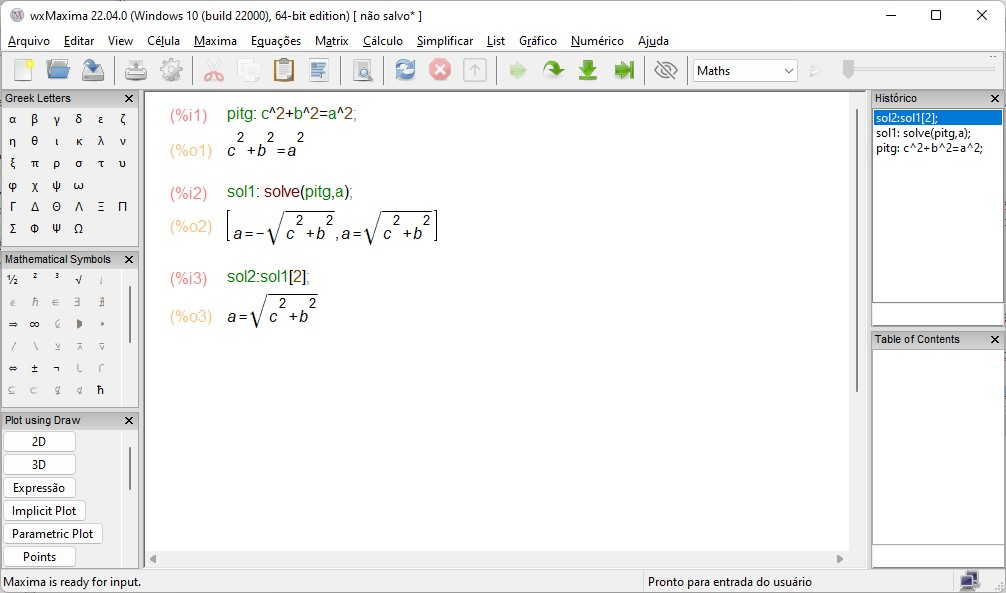
\includegraphics[scale=0.5]{pitagoras-5.jpg}
	%\end{Center}
\end{figure}
%%%

\noindent Observe que o Maxima atribuiu à expressão \textsf{sol2} o valor do segundo elemento do vetor \textsf{sol1}, ou seja, o valor do elemento de índice \textsf{[2]}

O Maxima também suporta um ambiente de texto, misturado entre os comandos algébricos, recurso muito útil no caso de o usuário precisar de documentar seu trabalho com texto explicativo e formatado. Por exemplo vamos colocar um título introdutório em nossa tela e uma texto explicativo intermediário. 

\noindent O título será um texto a ser inserido antes da primeira célula. Uma célula é o espaço delimitado pelo seletor lateral (parentese ``exótico'' que aparece à esquerda das expressões) idêntico ao desenho abaixo
\begin{figure}[hp]
	\centering
	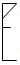
\includegraphics[scale=0.8]{seletor.jpg}
	\label{fig:seletor}
\end{figure}

\noindent O cursor horizontal deve ser transportado com auxílio das teclas de navegação do teclado, ou diretamente com o uso de dispositivo apontador (``mouse''), ver figura \ref{fig:curso-hrizontal-2}. 

\begin{figure*}[H]
	\centering
	\caption{Posição sugerida para escrever um título}
	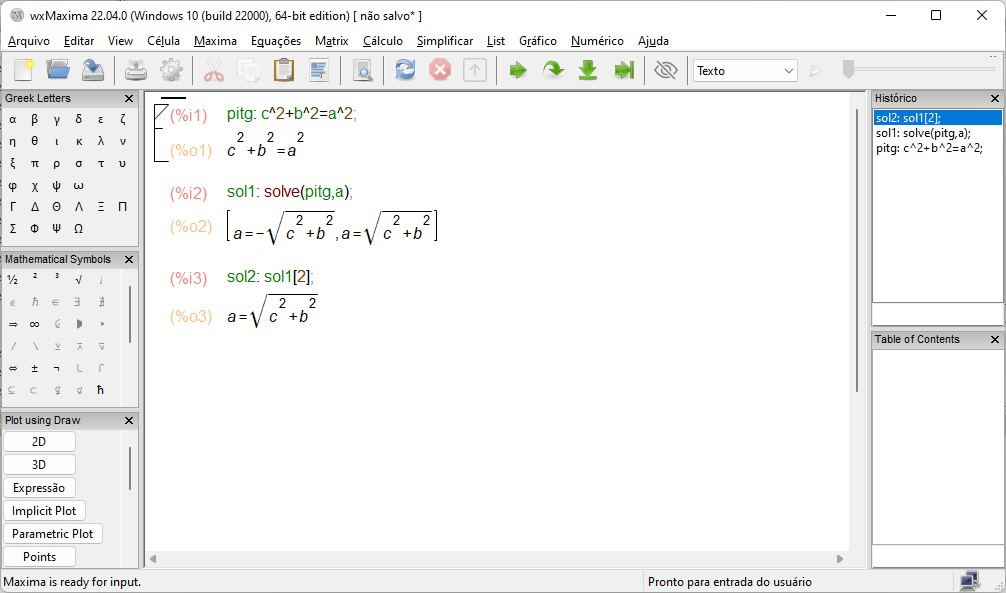
\includegraphics[width=0.80\textwidth]{curso-hrizontal-2.jpg}
	\label{fig:curso-hrizontal-2}
\end{figure*}

Em seguida digita-se o texto pretendido para título:
\begin{figure}[h]
	\centering
	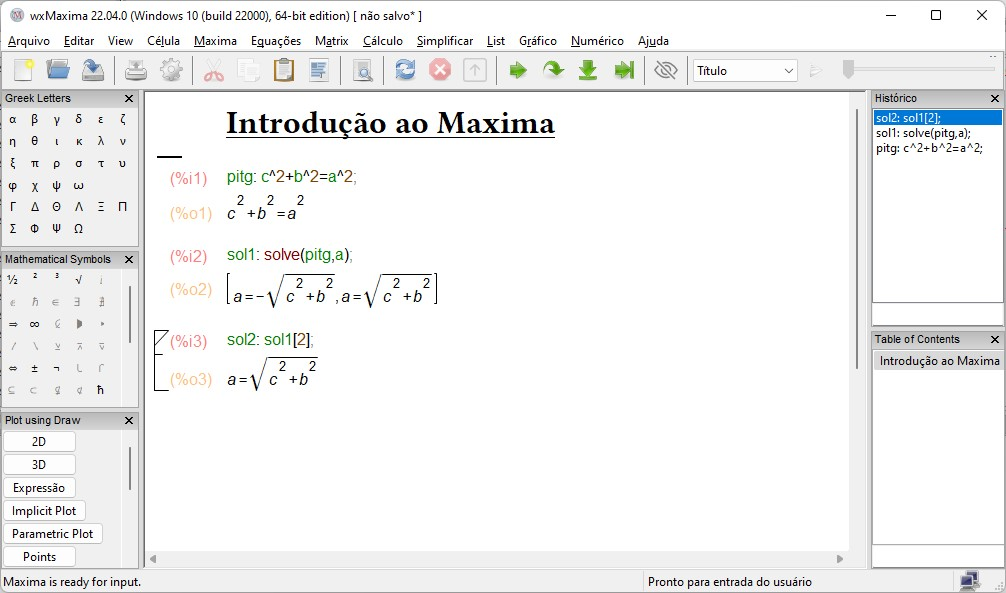
\includegraphics[width=0.80\textwidth]{introducao-maxima.jpg}
	\caption{Resultado da inserção de título}
	\label{fig:introducao-maxima}
\end{figure}
\clearpage

E, digita-se um texto explicativo pretendido:
\begin{figure}[ht!]
	\centering
	\caption{Resultado da inserção de texto comum}
	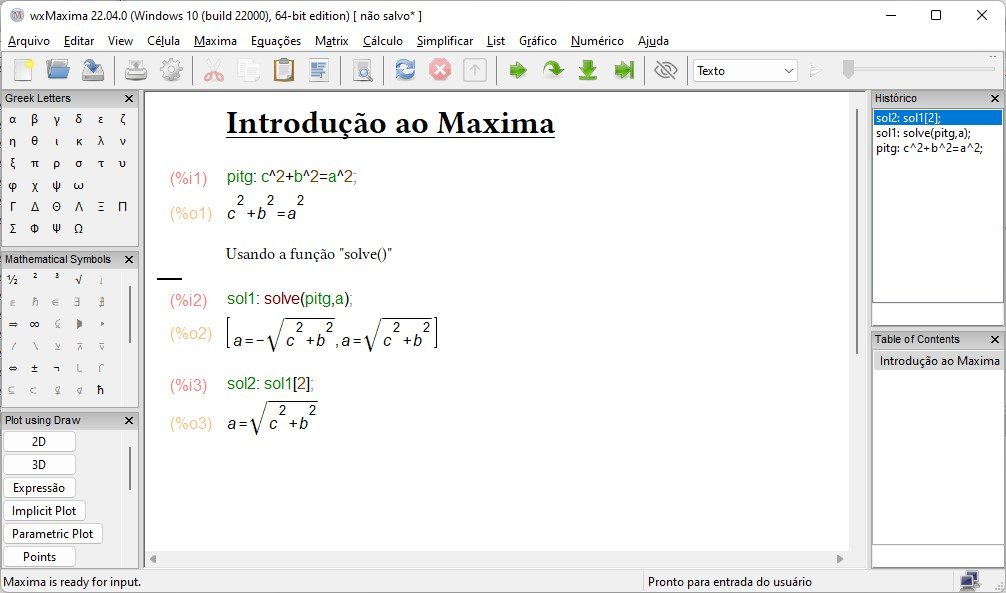
\includegraphics[width=0.80\textwidth]{usando-solve.jpg}
	\label{fig:usando-solve}
\end{figure}

Alguns elementos da estrutura do Maxima são estratégicos, como os \emph{flags}. Os \emph{flags} são os valores que determinadas variáveis internas do Maxima assumem de forma padrão ou conforme a definição do usuário. Exemplos:
\begin{itemize}
	\item {\texttt{showtime}} Tem valor \emph{false} como padrão. Quando definida para o valor \emph{true}, o tempo de processamento é impresso conjuntamente com cada saída de resultado.
	\begin{figure}[ht!]
		\centering
		\caption{Resultado obtido após aplicar configuração \emph{showtime}.}
		\label{fig:showtime-fig}
		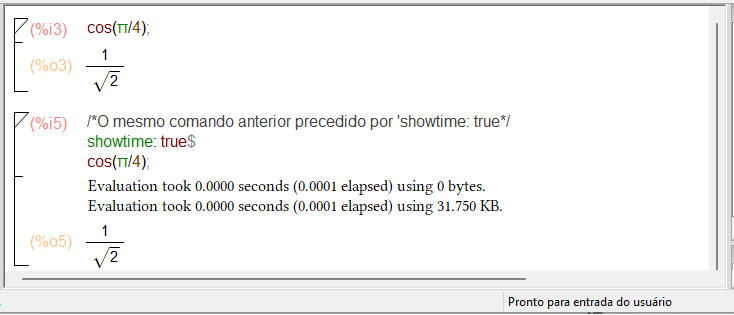
\includegraphics[width=0.7\linewidth]{showtime-fig}
	\end{figure}
	\item {\texttt{display2d}} Tem valor \emph{true} como padrão. Quando definido como  \emph{true} isso faz com que o Maxima apresente as expressões matemáticas na sua forma como as vemos nos livros.
	\begin{figure}[H]
		\centering
		\caption[]{Uso do variável \emph{display2D}}
		\label{fig:display-2d}
		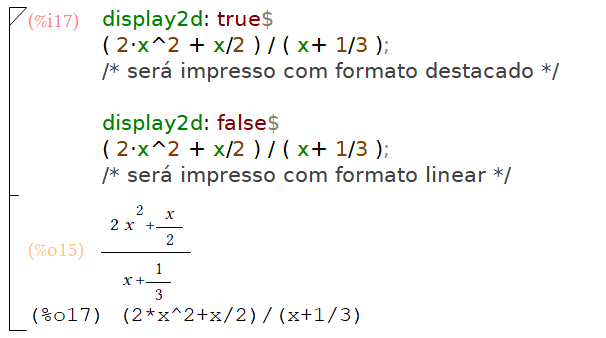
\includegraphics[width=0.7\linewidth]{display-2d}
	\end{figure}
	\item{\texttt{powerdisp}} Quando definido como true expõe os termos de uma soma em ordem crescente de suas potências.
\begin{figure}[H]
	\centering
	\caption{Demonstração do flag \emph{powerdisp}.}
	\label{fig:powerdisp}
	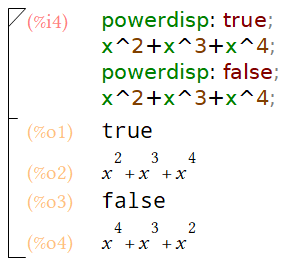
\includegraphics[width=0.4\linewidth]{powerdisp}
\end{figure}
\section{Listas e Matrizes}
Uma lista é usualmente uma coleção ou conjunto de dados com um significado específico. No Maxima uma lista deve ser entrada iniciando com o operador \([\) e finalizada com o \(]\).  Os elementos da lista devem estar separados por sinal de vírgula. A posição ordinal de cada elemento é relevante para efeitos de manipulação da lista, ou seja, para localizar um elemento basta fazer referência à sua posição ordinal na lista.
\begin{figure}[H]
	\centering
	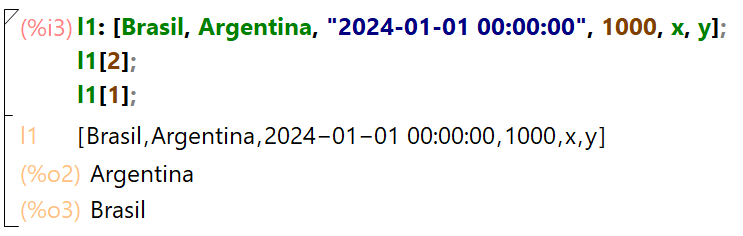
\includegraphics[width=0.7\linewidth]{listaexemplo1}
	\caption{Uma lista de dados entrada e apresentada no wxMaxima.}
	\label{fig:listaexemplo1}
\end{figure}

O funcionamento do Maxime é fortemente baseado no processamento em listas e saber trabalhar com lista é fundamental, eis alguns comandos que serão importantes já conhecê-los.
\begin{figure}[H]
	\centering
	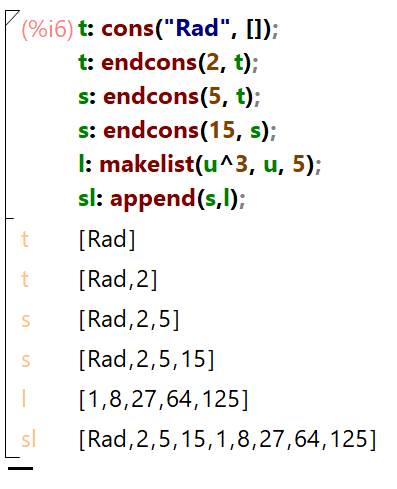
\includegraphics[width=0.4\linewidth]{listaexemplo2}
	\caption{Comantos para manipulação de listas no Maxima.}
	\label{fig:listaexemplo2}
\end{figure}

\end{itemize}
\section{Construção de Gráficos}
A construção de gráficos por intermédio do wxMaxima consiste na execução das funções de gráfico, que já estão embutidas como comandos da barra de menus.


O gráfico pode ser gerado em referência a um label de saída (\%o) ou mesmo uma entrada direta no campo da janela secundária da função de gráfico acionada pelo comando de menu.

Gráfico 2D 

\begin{figure}[ht]
	\centering
	\caption{Gráfico 2D a partir do comando do menu}
	\includegraphics[trim={0 10cm 0 0}, clip=true, width=0.7\linewidth]{"elementos de imagens fundamentos de gnuplot/screenshot005"}
\end{figure}

\begin{figure}[ht]
	\centering
	\caption{Entrando uma expressão rotulada}
	\label{fig:screenshot006}
	\includegraphics[trim={0 5cm 0 0}, clip=true,width=0.7\linewidth]{"elementos de imagens fundamentos de gnuplot/screenshot006"}
\end{figure}

\begin{figure}[ht]
	\centering
	\caption{Instruir no campo \emph{Format} para o wxMaxima para desenhar o gráfico na mesma janela da planilha}
	\label{fig:screenshot007}
	\includegraphics[trim={0 5cm 0 0}, clip=true,width=0.7\linewidth]{"elementos de imagens fundamentos de gnuplot/screenshot007"}
\end{figure}

\begin{figure}[ht]
	\centering
	\caption{Configurando para incluir quadrículas}
	\label{fig:screenshot008}
	\includegraphics[trim={0 5cm 0 0}, clip=true,width=0.7\linewidth]{"elementos de imagens fundamentos de gnuplot/screenshot008"}
\end{figure}

\begin{figure}[ht]
	\centering
	\caption{Finalizando essa entrada de dados para gerar o gráfico}
	\label{fig:screenshot009}
	\includegraphics[trim={0 5cm 0 0}, clip=true,width=0.7\linewidth]{"elementos de imagens fundamentos de gnuplot/screenshot009"}
\end{figure}

\begin{figure}[ht]
	\centering
	\caption{O gráfico está gerado e apresentado na planilha}
	\label{fig:screenshot010}
	\includegraphics[width=0.7\linewidth]{"elementos de imagens fundamentos de gnuplot/screenshot010"}
\end{figure}
\clearpage
Se fosse selecionada a opção \emph{gnuplot}, seria gerado o mesmo gráfico, porém em uma janela a parte, como mostrado na figuras a seguir.

\begin{figure}[ht]
	\centering
	\caption{Saída de gráfico por janela separada}
	\label{fig:screenshot011}
	\includegraphics[trim={0 5cm 0 0}, clip=true,width=0.7\linewidth]{"elementos de imagens fundamentos de gnuplot/screenshot011"}
\end{figure}

\begin{figure}[H]
	\centering
	\caption{Percorrendo agora a mesma sequência de configurações}
	\label{fig:screenshot012}
	\includegraphics[trim={0 5cm 0 0}, clip=true,width=0.7\linewidth]{"elementos de imagens fundamentos de gnuplot/screenshot012"}
\end{figure}

\begin{figure}[H]
	\centering
	\caption{Finalizando formato gnuplot}
	\label{fig:screenshot013}
	\includegraphics[trim={0 5cm 0 0}, clip=true,width=0.7\linewidth]{"elementos de imagens fundamentos de gnuplot/screenshot013"}
\end{figure}

\begin{figure}[H]
	\centering
	\caption{A figura mostra o gráfico em detalhe na janela gnuplot}
	\label{fig:screenshot014}
	\includegraphics[width=0.7\linewidth]{"elementos de imagens fundamentos de gnuplot/screenshot014"}
\end{figure}


Por hora esses são os conhecimentos sobre o Maxima, indispensáveis para imergir no universo de possibilidades. São conhecimentos básicos e no decorrer dos capítulos estaremos apresentando outros recursos, básicos ou mais complexos, conforme a exigência do contexto.


\chapter{ESTUDO DAS FUNÇÕES TRIGONOMÉTRICAS}
\label{estudos}
\newcounter{exemplos}
\setcounter{exemplos}{1}
\newcounter{exercicios}
\setcounter{exercicios}{1}
As funções trigonométricas tiveram suas origens no estudo das medidas astronômicas, e elas são de suma importância para as ciências em geral, dado que as suas características permitem de serem utilizadas para representar o comportamento de diversos sistemas reais. 

Elas são desenvolvidas por meio do estudo da circunferência de raio unitário com relação às dimensões em um determinado sistema de cordas. A palavra \emph{seno} etimologicamente significa meia corda. As funções trigonométricas também tem relações  com a geometria por meio das razões trigonométricas no triângulo retângulo.

As funções trigonométricas são ditas \emph{periódicas}. Uma função \(f:\mathds{R} \rightarrow \mathds{R}\) é dita periódica com período \(T > 0\)  se:
\begin{enumerate}{ }{ }
	\item  seu domínio contém \(x+T\) sempre que contém \(x\), e se
	\item \(f(x)=f(x+T)\) para todo \(x\) pertencente ao domínio de \(f\).
\end{enumerate}

\section{As Funções Trigonométricas no Maxima}
O Maxima usa \(:=\) para definir funções. Você irá se referir às trigonométricas usando as seguintes sintaxes.
\begin{itemize}
	\item seno: \textsf{f(u):=sin(u)};
	\item cosseno: \textsf{f(u):=cos(u)};
	\item tangente: \textsf{f(u):=tan(u)},
\end{itemize}
onde \emph{u}, ou seja, o argumento deve ser entendido como medida de arco expressa em radianos. 

\begin{minipage}[t]{\textwidth}\color{blue}
	\centering
	\noindent
	\texttt{CODE CELL MAXIMA}
\end{minipage}
\rule{\linewidth}{.1em}

\noindent
%%%%%%%%
%% INPUT:
\begin{minipage}[t]{4.000000em}\color{red}\bfseries
	--\ensuremath{\ensuremath{>}}	
\end{minipage}
\begin{minipage}[t]{\textwidth}\color{blue}
	/*\ Seno\ */\ \ \ f(x):=\ sin(x);\\
	/*\ Cosseno\ */\ \ g(x):=\ cos(x);\\
	/*\ Tangente\ */\ \ h(x):=\ tan(x);\\
	
\end{minipage}

\noindent%
\begin{figure}[H]
	\centering
	\label{fig:funcoestrig}
	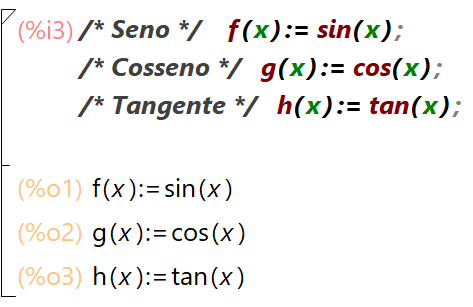
\includegraphics[width=0.4\linewidth]{funçõestrig}
\end{figure}

Outras funções trigonométricas.

\noindent
\begin{minipage}[t]{\textwidth}\color{blue}
	\centering
	\noindent
	\texttt{CODE CELL MAXIMA}
\end{minipage}
\rule{\linewidth}{.1em}



\noindent
%%%%%%%%
%% INPUT:
\begin{minipage}[t]{4.000000em}\color{red}\bfseries
	--\ensuremath{\ensuremath{>}}	
\end{minipage}
\begin{minipage}[t]{\textwidth}\color{blue}
	/*\ Secante\ */\ f(t):=\ sec(t);\\
	/*\ Cossecante\ */\ f1(k):=\ csc(k);\\
	/*\ Cotangente\ */\ k(k):=\ cot(k);\\
	/*\ exemplos:\ */\\
	k:\ 3;\ 'k(k)\ =\ k(k);\\
	numer:\ false\$\ 'f(t:10)\ =\ f(t:10);\\
	numer:\ true\$\ 'f(t:10)\ =\ f(t:10);\\
	'f1(1)\ =\ f1(1);
\end{minipage}

\noindent%


\begin{figure}[H]
	\centering
	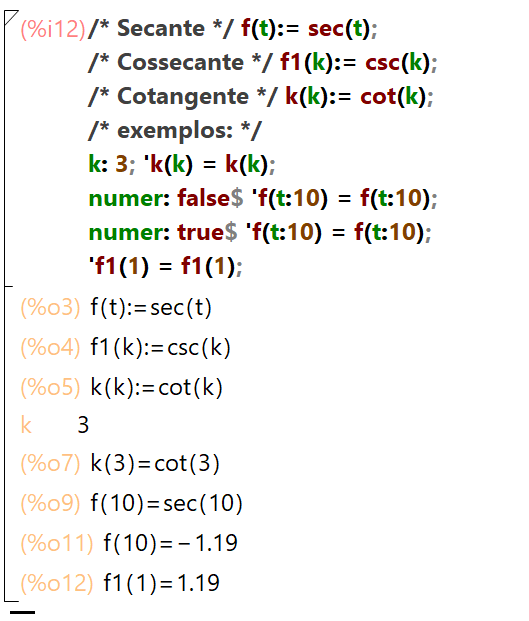
\includegraphics[width=0.5\linewidth]{funçãoHarmônica2}
	\label{fig:funcaoharmonica2}
\end{figure}

%Constante pi
A constante \(\pi\), utilizada na trigonometria é representada pelo comando \%pi. Como exemplo vamos calcular o seno de \({5 \pi \over 12}\).
\noindent\\
\begin{minipage}[t]{\textwidth}\color{blue}
	\centering
	\noindent
	\texttt{CODE CELL MAXIMA}
\end{minipage}
\rule{\linewidth}{.1em}
\noindent
%% constante pi:
\begin{minipage}[t]{4.000000em}\color{red}\bfseries
	--\ensuremath{\ensuremath{>}}	
\end{minipage}
\begin{minipage}[t]{\textwidth}\color{blue}
	kill(all)\$\\
	\ensuremath{\alpha}:\ 3*\%pi/12\$\\
	\ensuremath{\beta}:\ 2*\%pi/12\$\\
	\%piargs:\ true\$\ /*\ para\ usar\ o\ valor\ de\ \ensuremath{\pi}\ */\\
	t:\ \ [\ sin(\ensuremath{\alpha}),\ cos(\ensuremath{\alpha}),\ sin(\ensuremath{\beta}),\ cos(\ensuremath{\beta})\ ]\$\\
	t:\ensuremath{\sim\ }rat(\ t[1]*t[4]+\ t[2]*t[3]\ )\$\\
	\%piargs:\ false\$\ /*\ para\ mostrar\ símbolo\ \ensuremath{\pi}\ */\\
	disp('sin(\ensuremath{\alpha}+\ensuremath{\beta})\ =\ t)\$
\end{minipage}

\noindent%

\begin{figure}[H]
	\centering
	%\caption{}
	\label{fig:uso-dao-rat1}
	\includegraphics[width=0.6\linewidth]{"uso dao rat1"}
\end{figure}


Em muitas aplicações trigonométricas seus argumento são constituídos de  funções compostas.

\noindent
\begin{minipage}[t]{\textwidth}\color{blue}
	\centering
	\noindent
	\texttt{CODE CELL MAXIMA}
\end{minipage}
\rule{\linewidth}{.1em}


\noindent
%%%%%%%%
%% INPUT:
\begin{minipage}[t]{4.000000em}\color{red}\bfseries
	--\ensuremath{\ensuremath{>}}	
\end{minipage}
\begin{minipage}[t]{\textwidth}\color{blue}
	kill(all)\$\\
	f(x):=\ sin(a*x\ +\ b);\\
	g(x):=f(x)\^\ 2;\\
	h(x):=f(x)*\ sin(a\_1*x\ +\ b\_1);\\
	f(1);\\
	'g(1)\ =\ g(1)\ ;\\
	h(\%pi/2);\\
	f(x)+g(x);\\
	'f(x)+'g(x)\ =\ f(x)+g(x);
\end{minipage}

\noindent%
\begin{figure}[H]
	\centering
	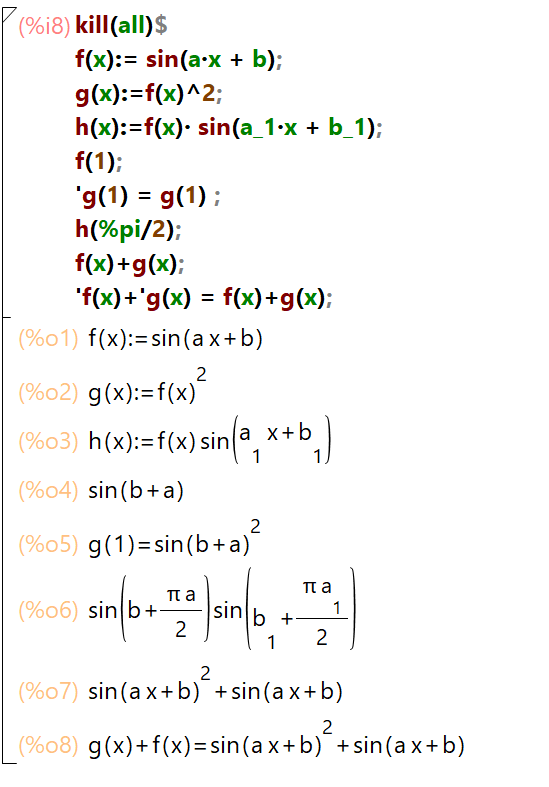
\includegraphics[width=0.5\linewidth]{funçãoHarmônica3}
	\label{fig:funcaoharmonica3}
\end{figure}


As funções trigonométricas podem ser manipuladas de forma simbólica e de forma numérica.

\noindent
\begin{minipage}[t]{\textwidth}\color{blue}
	\centering
	\noindent
	\texttt{CODE CELL MAXIMA}
\end{minipage}
\rule{\linewidth}{.1em}
\noindent
\begin{minipage}[t]{4.000000em}\color{red}\bfseries
	--\ensuremath{\ensuremath{>}}	
\end{minipage}
\begin{minipage}[t]{\textwidth}\color{blue}
	kill(all)\$\ numer:\ false\$\ \%piargs:\ true\$\ \ensuremath{\alpha}:\ \%pi/12\$\ ARCO:\ [\ \ensuremath{\alpha},\ 2*\ \ensuremath{\alpha},\ 3*\ensuremath{\alpha},\ 4*\ensuremath{\alpha}]\$\\
	block(\ i:\ 1,\ loop1,\ \ \ensuremath{\alpha}:\ \%pi/12,\ arco:\ [\ \ensuremath{\alpha},\ 2*\ \ensuremath{\alpha},\ 3*\ensuremath{\alpha},\ 4*\ensuremath{\alpha}],\ \\
	\ \ \ \ seno:\ append(["Seno"],\ makelist(sin(\ensuremath{\alpha}),\ \ensuremath{\alpha},\ arco)),\\
	\ \ \ \ cosseno:\ append(["Cosseno"]\ \ ,\ makelist(cos(\ensuremath{\alpha}),\ \ensuremath{\alpha},\ arco)),\\
	\ \ \ \ tangente:\ append(["Tangente"],\ makelist(tan(\ensuremath{\alpha}),\ \ensuremath{\alpha},\ arco)),\\
	\ \ \ \ matriz:\ matrix(append(["ARCO"],\ ARCO),\ seno,\ cosseno,\ tangente),\\
	\ \ \ \ disp("Formato\ de\ tabela.",\ matriz),\ \\
	\ \ \ \ numer:\ true,\ fpprintprec:\ 3,\ i:\ i+1,\ \ if\ i\ensuremath{<}3\ then\ go(loop1)\\
	)\$
\end{minipage}

\noindent%

%formato de tabela figura
\begin{figure}[H]
	\centering
	%\caption{}
	\label{fig:formatodetabela}
	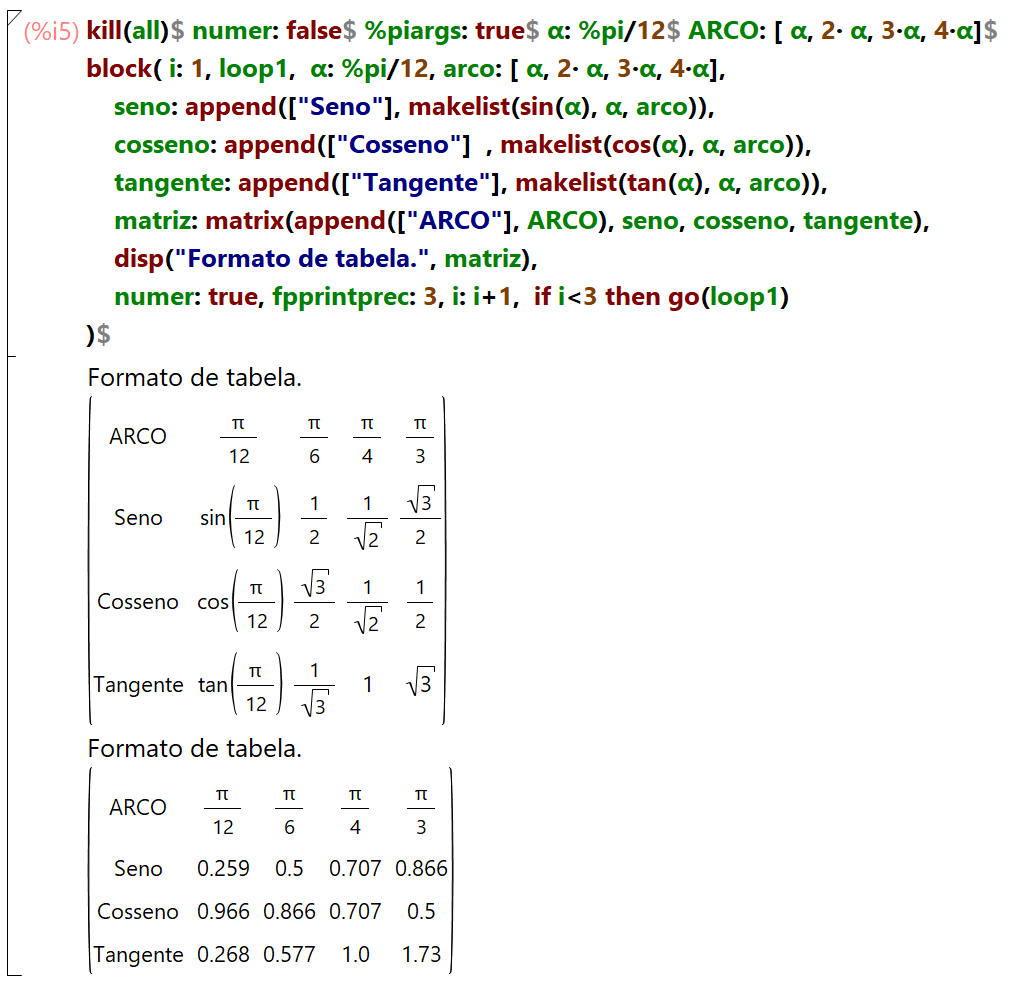
\includegraphics[width=.9\linewidth]{formatodetabela}
\end{figure}
 
 \section{Transformações Trigonométricas}
São relações trigonométricas para as operações com arcos. Temos então que, dados dois arcos $\alpha$ e $\beta$ temos as seguintes identidades trigonométricas:
\begin{align*}
	\sin\qty(\alpha+ \beta)\,&=\, \sin\alpha \, \cos\beta + \cos\alpha\, \sin\beta\\
	\cos\qty(\alpha + \beta )\,&=\, \cos\alpha \, \cos \beta - \sin\alpha\, \sin\beta \text{.}
\end{align*}
Essa forma explícita da soma dos arcos são alcançadas usando a função \texttt{trigexpand}.

\begin{minipage}[t]{\textwidth}\color{blue}
	\centering
	\noindent
	\texttt{CODE CELL MAXIMA}
\end{minipage}
\rule{\linewidth}{.1em}
\noindent
%%%%%%%%
%% INPUT:
\begin{minipage}[t]{4.000000em}\color{red}\bfseries
	--\ensuremath{\ensuremath{>}}	
\end{minipage}
\begin{minipage}[t]{\textwidth}\color{blue}
	kill(all)\$\\
	exp1:\ cos(\ensuremath{\alpha}+\ \ensuremath{\beta});
\end{minipage}
\noindent%
\begin{figure}[H]
	\centering
	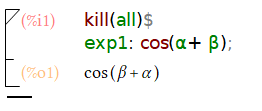
\includegraphics[width=0.35\linewidth]{dica-trigexpand1}
	%\caption{}
	\label{fig:dica-trigexpand1}
\end{figure}

\noindent
%%%%%%%%
%% INPUT:
\begin{minipage}[t]{4.000000em}\color{red}\bfseries
	--\ensuremath{\ensuremath{>}}	
\end{minipage}
\begin{minipage}[t]{\textwidth}\color{blue}
	trigexpand(exp1);
\end{minipage}

\noindent%
\begin{figure}[H]
	\centering
	%\caption{}
	\label{fig:trigexpand2}
	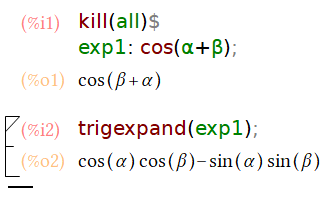
\includegraphics[width=0.4\linewidth]{trigexpand2}
\end{figure}
Usam-se as funções trigonométricas com o argumento arco metade, porém é preciso obedecer certar regras, como mostrado na dica a seguir usando os \emph{flags} \texttt{halfangles}, e \texttt{\%piargs}

\noindent
\begin{minipage}[t]{\textwidth}\color{blue}
	\centering
	\noindent
	\texttt{CODE CELL MAXIMA}
\end{minipage}
\rule{\linewidth}{.1em}

\noindent
%%%%%%%%
%% INPUT:
\begin{minipage}[t]{4.000000em}\color{red}\bfseries
	--\ensuremath{\ensuremath{>}}	
\end{minipage}
\begin{minipage}[t]{\textwidth}\color{blue}
	\%piargs:\ true\$\\
	assume(\ensuremath{\alpha}\ensuremath{>}0,\ \ensuremath{\alpha}\ensuremath{<}2*\%pi)\$\\
	halfangles:\ false\$\\
	exp1:\ (sin(\ensuremath{\alpha}/2))\$\\
	halfangles:\ true\$\\
	exp1\ =\ sin(\ensuremath{\alpha}/2)\ ;
\end{minipage}

\noindent%
\begin{figure}[H]
	\centering
	%\caption{}
	\label{fig:halfangles}
	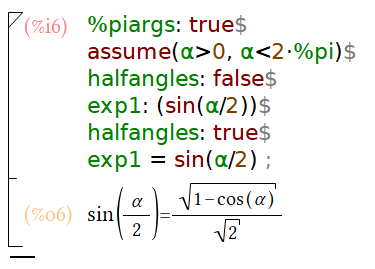
\includegraphics[width=0.4\linewidth]{halfangles}
\end{figure}

As funções trigonométricas de arco múltiplo também são possíveis de serem expandidas usando o \texttt{trigexpand}.

\noindent
\begin{minipage}[t]{\textwidth}\color{blue}
	\centering
	\noindent
	\texttt{CODE CELL MAXIMA}
\end{minipage}
\rule{\linewidth}{.1em}
\noindent
\begin{minipage}[t]{4.000000em}\color{red}\bfseries
	--\ensuremath{\ensuremath{>}}	
\end{minipage}
\begin{minipage}[t]{\textwidth}\color{blue}
	kill(all)\ \$\\
	/*\ números\ inteiros\ */\ m:\ [2,3,4,5]\$\ \\
	\\
	trigexpand:\ \ false\ \$\\
	exp1:\ sin(m*\ensuremath{\alpha})\ \$\\
	trigexpand:\ \ true\ \$\\
	for\ i:\ 1\ thru\ 4\ do\ \\
	\ \ \ \ (\\
	\ \ \ \ \ \ \ \ display\ (exp1[i]\ =\ sin(m[i]*\ensuremath{\alpha}))\\
	\ \ \ \ )\ \$
\end{minipage}
\noindent%
\begin{figure}[ht!]
	\centering
	%\caption{}
	\label{fig:arcomultiplo}
	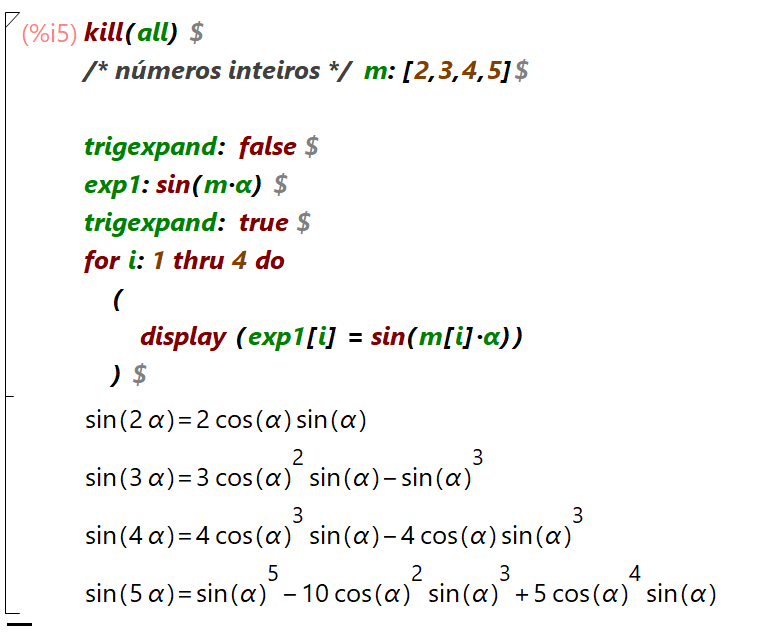
\includegraphics[width=0.7\linewidth]{arcomúltiplo}
\end{figure}
\newpage
Algumas funcionalidade permitem obter identidade trigonométricas

\noindent
\begin{minipage}[t]{\textwidth}\color{blue}
	\centering
	\noindent
	\texttt{CODE CELL MAXIMA}
\end{minipage}
\rule{\linewidth}{.1em}
\noindent
\begin{minipage}[t]{4.000000em}\color{red}\bfseries
	--\ensuremath{\ensuremath{>}}	
\end{minipage}
\begin{minipage}[t]{\textwidth}\color{blue}
	eq1:\ 2*\ sin((\ensuremath{\alpha}-\ensuremath{\beta})\ /2\ )\ *\ \ cos((\ensuremath{\alpha}+\ensuremath{\beta})\ /2\ )\$\\
	eq2:\ \ trigrat\ (eq1)\ \$\\
	display(\ \ eq2\ =\ eq1)\$
\end{minipage}

\noindent%
\begin{figure}[ht]
	\centering
	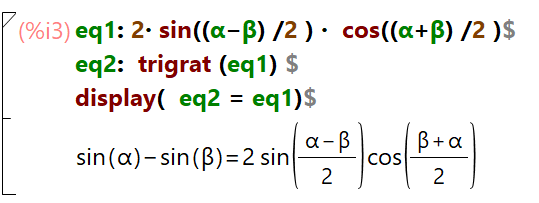
\includegraphics[width=0.5\linewidth]{identidade}
	%\caption{}
	\label{fig:identidade}
\end{figure}

\clearpage
Copie na memória do seu computador as linhas de comando desse exemplo \thesection.\theexemplos\, e cole-as na janela do wxMaxima, avalie com o comando de teclado \texttt{Shift+Enter} e veja o resultado, deverá ser idêntico ao da figura \ref{fig:exemplo331}. O conteúdo limitado entre '/* */' é interpretado apenas como texto de comentários.

%%% pesquisar evfun no maxima  - distribute_over	- cabs - Trigonometric functions
%%%
\begin{tcolorbox}[enhanced jigsaw, colback=gray!30, colframe=Maroon,width=1\textwidth, arc=3mm, auto outer arc, boxrule=5pt, drop shadow={Maroon!50!gray!80}]
	\noindent
	Exercício \thesection.\theexercicios: No código abaixo acrescente ou modifique comandos de forma que apareçam,
	\begin{enumerate}
		\item uma linha, correspondente aos valores de secante e, 
		\item uma coluna, ao arco igual a $\frac{5\,\pi}{12}$.
	\end{enumerate}
	\noindent
	\begin{minipage}[t]{\textwidth}\color{blue}
		\centering
		\noindent
		\texttt{CODE CELL MAXIMA}
	\end{minipage}
	\rule{\linewidth}{.1em}
	\noindent
	\begin{minipage}[t]{4.000000em}\color{red}\bfseries
		--\ensuremath{\ensuremath{>}}	
	\end{minipage}
	\begin{minipage}[t]{\textwidth}\color{blue}
		kill(all)\$\ numer:\ false\$\ \%piargs:\ true\$\ \ensuremath{\alpha}:\ \%pi/12\$\ ARCO:\ [\ \ensuremath{\alpha},\ 2*\ \ensuremath{\alpha},\ 3*\ensuremath{\alpha},\ 4*\ensuremath{\alpha}]\$\\
		block(\ i:\ 1,\ loop1,\ \ \ensuremath{\alpha}:\ \%pi/12,\ arco:\ [\ \ensuremath{\alpha},\ 2*\ \ensuremath{\alpha},\ 3*\ensuremath{\alpha},\ 4*\ensuremath{\alpha}],\ \\
		\ \ \ \ seno:\ append(["Seno"],\ makelist(sin(\ensuremath{\alpha}),\ \ensuremath{\alpha},\ arco)),\\
		\ \ \ \ cosseno:\ append(["Cosseno"]\ \ ,\ makelist(cos(\ensuremath{\alpha}),\ \ensuremath{\alpha},\ arco)),\\
		\ \ \ \ tangente:\ append(["Tangente"],\ makelist(tan(\ensuremath{\alpha}),\ \ensuremath{\alpha},\ arco)),\\
		\ \ \ \ matriz:\ matrix(append(["ARCO"],\ ARCO),\ seno,\ cosseno,\ tangente),\\
		\ \ \ \ disp("Formato\ de\ tabela.",\ matriz),\ \\
		\ \ \ \ numer:\ true,\ fpprintprec:\ 3,\ i:\ i+1,\ \ if\ i\ensuremath{<}3\ then\ go(loop1)\\
		)\$
	\end{minipage}
\end{tcolorbox}
%%%


\chapter{DESCRIÇÕES DE MOVIMENTOS ONDULATÓRIOS}
Há várias situações no dia a dia nas quais as coisas acontecem repentinamente, ou inesperadamente, vindo, depois a cessar seus efeitos, ou, em outros casos, repercutem mais além. É comum nos referirmos a isso com a expressão: ``isso é apenas uma onda, logo passará''. Isso, claro, devido a que tais situações são transitórias, exemplos: pandemias, endemias, o preço de commodities, tsunamis, terremotos, até notícias ou eventos cotidianos. Algumas vezes tais situações apresentam comportamento oscilante, como na superfície de um líquido em uma piscina, ou mesmo em fontes naturais de água, como em rios, mares e oceanos durante a passagem de uma embarcação.

É importante notar que existem características diferentes em tais situações. Alguns simplesmente oscilam ou vibram e em outros casos, além de oscilar ou vibrar, essa condição é posteriormente transmitida para outros locais do ambiente onde tais situações ocorrem. Neste segundo caso, diz-se que há uma propagação do fenômeno. De tal forma que, oscilação, onda, propagação são termos correlacionados e condicionam a natureza do movimento ondulatório de interesse da física.

\section{O Movimento Ondulatório}
Vamos supor uma haste fina de metal em que alguém bata com uma ferramente sobre sua extremidade então outra pessoa oposta sentirá as vibrações dos impactos cujo efeito seria, dada sua elasticidade, devido a sucessão de pequenos movimentos MHS sobre extremidade observada. Porém, na medida em que as estocadas forem mais intensas parte da energia fornecida será acumulada localmente na haste originando uma sucessão de movimentos abruptos avançando pela extensão até isso ser percebido na extremidade oposta. Ou seja, nessa condição houve uma transferência de energia inicialmente acumulada na elasticidade de uma seção do material, na forma de um \emph{pacote} e que por efeito secundário entrou em propagação nas seções subsequente. Esse movimento da energia assim descrito é tipicamente ondulatório.

O movimento ondulatório compreende tudo que ocorre como consequência de uma perturbação que se propaga além de seu local e com a condição de apresentar nisso inerentes efeitos de difração e interferência. Nesse sentido, e uma vez que se estabeleça um sistema de referência, então, um observador, sob a perspectiva de um experimento ou uma hipótese, descreverá seus resultados por meio de uma terminologia, a qual traduz, de certa forma, as propriedades do movimento ondulatório:
\begin{itemize}
	\item A \emph{perturbação}, que é a ação inicial, intencional ou não, que leva a efeito a produção do que vem a ser uma onda. O local onde houve a perturbação marca origem ou a \emph{fonte}. Então uma onda diz-se que é \emph{produzida}.
	\item Uma vez que a ação perturbatória resultou em uma onda sobre o meio ou campo então essa onda é chamada de um \emph{pulso}. O pulso é \emph{enviado} e possui perspectiva de direção, tempo e espaço. Portanto o pulso viaja ou caminha.
	\item A atuação contínua da perturbação leva a efeito uma sucessão de pulsos, ou \emph{trem de ondas}. A ação periódica da fonte gera um \emph{trem de ondas periódico}.
	\item Todos os pontos do meio ou campo sujeitos a uma mesma onda possuem o mesmo \emph{estado de movimento}. Tais pontos constituem uma \emph{frente de onda}
	
	\item A curva ou superfície decorrente da frente de onda define o \emph{perfil da frente de onda}. Os perfis de onda podem ser descritos por meio de funções matemáticas.
%
	\item A direção é um aspecto importante na descrição do movimento ondulatório e, como a frente de onda possui uma conotação geométrica, reside sobre ela o conceito de \emph{raio}, que é uma linha reta perpendicular à curva ou superfície definida pela frente de onda. O raio indica a \emph{direção do movimento ondulatório} ou de \emph{propagação}.
%
	\item As partículas do meio ou linhas de campo afetadas pelo pulso ou onda efetuam apenas deslocamento temporário ou oscilação em torno de sua posição original ou de equilíbrio,                                                                                                                                                                                                                                                                                                                                                                                                                                                                                                                                                                                                                                                                                                                                                                                                                                                                                                                                                                                                                                                                                                                                                                                                                                                                                                                                                                                                                                                                                                                                                                                                                                                                                                                                                                                                                                                                                                                                                                                                                                                                                                                                                                                                                                                                                                                                                                                                                                                                                                                                                                                                                                                                                                                                                                                                                                                                                                                                                                                                                                                                                                                                                                                                                                                                                                                                                                                                                                                                                                                                                                                                                                                                                                                                                                                                                                                                                                                                                                                                                                                                                                                                                                                                                                                                                                                                                                                                                                                                                                                                                                                                                                                                                                                                                                                                                                                                                                                                                                                                                                                                                                                                                                                                                                                                                                                                                                                                                                                                                                                                                                                                                                                                                                                                                                                                                                                                                                                                                                                                                                                                                                                                                                                                                                                                                                                                                                                                                                                                                                                                                                                                                                                                                                                                                                                                                                                                                                                                                                                                                                                                                                                                                                                                                                                                                                                                                                                                                                                                                                                                                                                                                                                                                                                                                                                                                                                                                                                                                                                                                                                                                                                                                                                                                                                                                                                                                                                                                                                                                                                                                                                                                                                                                                                                                                                                                                                                                                                                                                                                                                                                                                                                                                                                                                                                                                                                                                                                                                                                                                                                                                                                                                                                                                                                                                                                                                                                                                                                                                                                                                                                                                                                                                                                                                                                                                                                                                                                                                                                                                                                                                                                                                                                                                                                                                                                                                                                                                                                                                                                                                                                                                                                                                                                                                                                                                                                                                                                                                                                                                                                                                                                                                                                                                                                                                                                                                                                                                                                                                                                                                                                                                                                                                                                                                                                                                                                                                                                                                                                                                                                                                                                                                                                                                                                                                                                                                                                                                                                                                                                                                                                                                                                                                                       ou seja, não há um deslocamento resultante para elas. Portanto, a \emph{amplitude} se configura pela medida do deslocamento de um elemento do meio ou linha de campo submetido ao movimento perturbatório a partir da posição de equilíbrio.
%
	\item É de grande interesse para o estudo da Ondulatória o perfil \emph{senoidal} ou harmônico. O que leva a abordagem do \emph{estado da onda}, que pode ser
	\begin{itemize}
		\item estacionário;
		\item em propagação.
	\end{itemize}
	
	\item O \emph{tipo de onda} quanto ao seu princípio físico governante, que devem ser: \emph{ondas mecânicas},  \emph{eletromagnéticas} e \emph{materiais}.
\end{itemize}

Máxwell descobriu que o campo elétrico dependente do tempo propaga-se no vácuo e tal condição pode ser interpretada pela ondulatória. Tem-se portanto a teoria das ondas eletromagnéticas. Um dos mecanismo para a produção de ondas eletromagnética é o dipolo elétrico e um outro é magnético, ou seja são fontes desses tipos de onda.

\newpage
%%%%%%%%
\section{Abordagem Matemática} O movimento ondulatório está vinculado necessariamente à uma natureza perturbatória. Isso sugere abordagens matemáticas similares se considerarmos aspectos oscilatórios. Na física, oscilações tem como modelo matemático padrão o movimento harmônico simples (MHS), o qual é retratado como o deslocamento periódico de uma partícula em torno do seu ponto de equilíbrio medido como uma função senoidal do tempo. 

Se considerarmos tal situação de oscilação ocorrendo sobre o eixo X do plano cartesiano e em torno da origem então o deslocamento será
\begin{equation*}
	x\qty(t) = A\, \sin\omega\,t \text{.}
\end{equation*}
No caso mais geral de o movimento não se iniciar na origem então teremos
\begin{equation*}
	x(0) = A' \neq  0\text{,}
\end{equation*}
e como, nesse caso, \(\qty|A'|<\qty|A|\), então podemos fazer
\begin{equation*}
	x(0) = A\, \sin \alpha\text{,}
\end{equation*}
e assim a expressao mais geral seria
\begin{equation*}
	x\qty(t) = A\, \sin\qty(\omega\,t+ \alpha) \text{,}
\end{equation*}
onde o argumento \(\qty(\omega\,t+ \alpha)\) é um valor que se dá em radianos trigonométricos, inclusive, isso permite a representação do MHS pela técnica de \emph{vetor girante}. Isto é possível devido à relação que existe entre o movimento circular uniforme (MCU) e o oscilatório.


Na medida em que a perturbação oscilante esteja associada ao movimento ondulatório subsequente então podemos usar o MHS para representar seu perfil de onda. 

Seja então uma variável independente \(\theta\), em radianos, coincidindo com o eixo das abcissas do plano cartesiano, então teríamos a expressão da função seno na forma:
\begin{equation*}
	\xi \qty(\theta) =\xi_0 \sin\theta \text{,}
\end{equation*}

\noindent
% Code cell para função trigonométrica abordadem matemática
\begin{minipage}[t]{\textwidth}\color{blue}
	\centering
	\noindent
	\texttt{CODE CELL MAXIMA}
\end{minipage}
	\rule{\linewidth}{.1em}
\noindent
\begin{minipage}[t]{4.000000em}\color{red}\bfseries
	--\ensuremath{\ensuremath{>}}	
\end{minipage}
\begin{minipage}[t]{\textwidth}\color{blue}
	kill(all)\$\ \ \\
	declare\_subscripted(\ensuremath{\xi}\_0)\$\\
	disp(box(\ \ensuremath{\xi}(\ensuremath{\theta}):=\ \ \ensuremath{\xi}\_0\ *\ sin(\ensuremath{\theta})))\$
\end{minipage}

\noindent%

\begin{figure}[H]
	\centering
	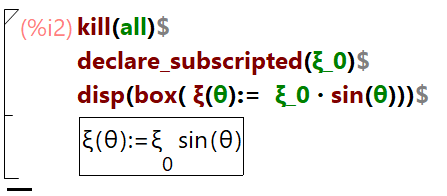
\includegraphics[width=0.4\linewidth]{funçãoHarmônica}
	\label{fig:funcaoharmonica}
\end{figure}
\noindent
onde, \( \xi\qty(\theta) \) é o valor da função, corresponde a uma ordenada ou cota, como na figura \ref{fig:geogebra-seno}, e que poderia estar representando a \emph{amplitude local} de uma propriedade física. E  o arco, \( \theta \), do qual está sendo calculado o seno, é \emph{a fase} onde se apresenta a evolução da onda. É um valor de arco representando um ponto sobre o eixo de propagação cuja a amplitude associada será sempre de mesmo valor à medida que se evolua a função \( \xi \) por meio de ciclos iguais a \( 2\,\pi\, \mathrm{rad} \), ou seja, $\Theta + 2\, \pi$ .

\noindent
% Code cell para função trigonométrica abordadem matemática
\begin{minipage}[t]{\textwidth}\color{blue}
	\centering
	\noindent
	\texttt{CODE CELL MAXIMA}
\end{minipage}
\rule{\linewidth}{.1em}
\noindent
\begin{minipage}[t]{4.000000em}\color{red}\bfseries
	--\ensuremath{\ensuremath{>}}	
\end{minipage}
\begin{minipage}[t]{\textwidth}\color{blue}
	kill(all)\$declare\_subscripted(\ensuremath{\xi}\_0)\$\ \ensuremath{\xi}(\ensuremath{\theta}):=\ \ensuremath{\xi}\_0*sin(\ensuremath{\theta})\$\ \ensuremath{\xi}\_0:\ [10,\ 15,-5]\$\ensuremath{\xi}(\ensuremath{\theta}):=\ \ensuremath{\xi}\_0[1]*sin(\ensuremath{\theta})\$\\
	wxdraw2d(\ axis\_top\ =\ false,\ axis\_bottom\ =\ false,\ xtics\_axis\ =\ true,\\
	\ \ \ \ explicit(\ensuremath{\xi}(\ensuremath{\theta}),\ensuremath{\theta},0,2*\%pi),\ explicit(0,\ensuremath{\theta},0,2*\%pi),\ explicit(\ensuremath{\xi}\_0[1],\ensuremath{\theta},0,2*\%pi),\\
	\ \ \ \ explicit(-\ensuremath{\xi}\_0[1],\ensuremath{\theta},0,2*\%pi),\ \ \ \ \ point\_type\ =\ filled\_circle,\ \ point\_size\ \ =\ 2,\ \\
	\ \ \ \ points\_joined\ =\ true,\ \ points([\ [2.5,\ensuremath{\xi}(2.5)],\ [2.5,0]\ ]),\ /*\ Ordenda\ da\ função\ em\ \ensuremath{\theta}\ */\\
	\ \ \ \ grid=[1,1],\ color\ =\ \_blue,\ font\ =\ "Arial",\ font\_size\ =\ 20,\\
	\ \ \ \ label([concat(\ "y\ =\ \ensuremath{\xi}\_0"),1,\ensuremath{\xi}\_0[1]-.2]\ ),\ label([concat(\ "y\ =\ -\ \ensuremath{\xi}\_0"),1,-\ensuremath{\xi}\_0[1]+.5]\ ),\\
	\ \ \ \ label([\ "\ensuremath{\theta}",\ \ \ \ 2.5,\ -0.5\ \ ]),\ \ label([concat(\ "\ensuremath{\xi}(\ensuremath{\theta})=",\ \ensuremath{\xi}\_0[1],\ "*sin(\ensuremath{\theta})"),\ \ 3.1,\ensuremath{\xi}(2.5)\ \ ])\ )\$
\end{minipage}

\noindent%
	\begin{figure}[H]
		\centering
		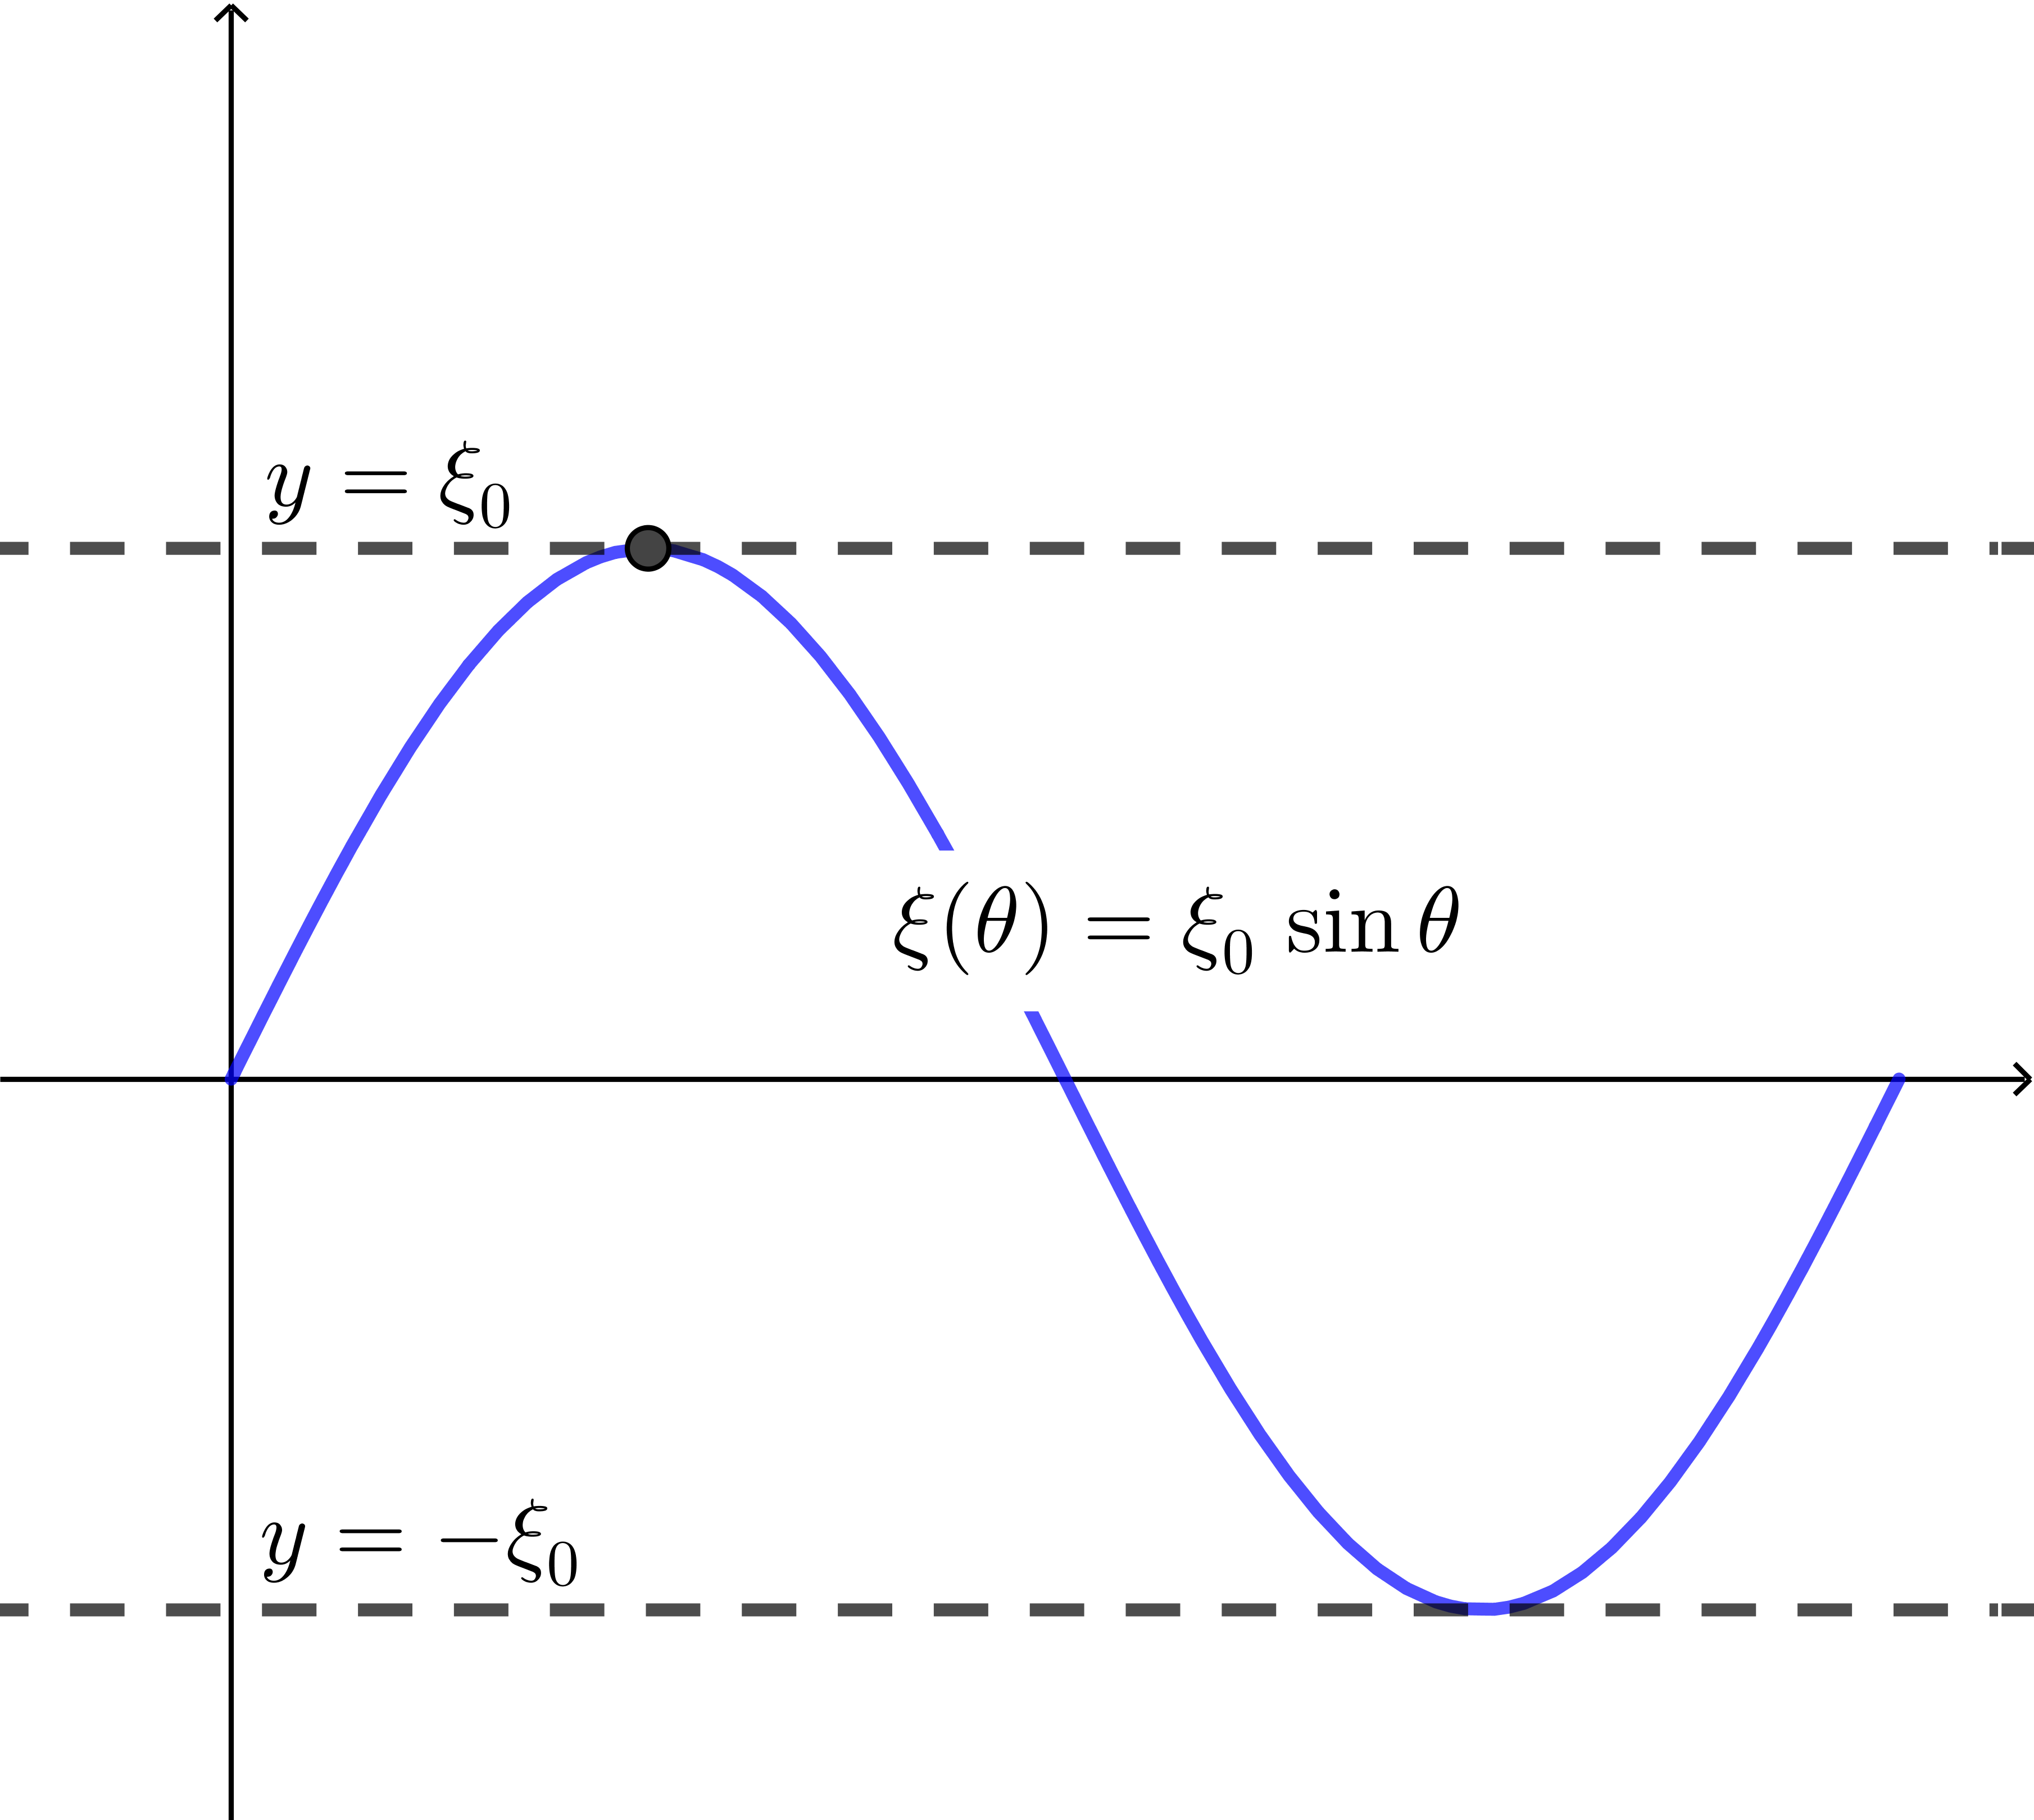
\includegraphics[scale=.5]{geogebra-seno}
		\caption[]{Perfil da função harmônica.}
		\label{fig:geogebra-seno}
	\end{figure}


Vamos supor que tenhamos agora uma outra função na forma
\begin{equation*}
	\xi_1 \qty(\theta) =\xi_0 \sin\qty(\theta- \delta)\text{.}
\end{equation*} Esta seria representada na forma do gráfico da figura \ref{fig:geogebra-seno-2}, ou seja, uma \emph{senoide} deslocada da origem dos eixos à direita.
\begin{figure}[H]
	\centering
	\caption[]{Gráfico de um perfil de uma função harmônica deslocado da origem do eixo das abcissas.}
	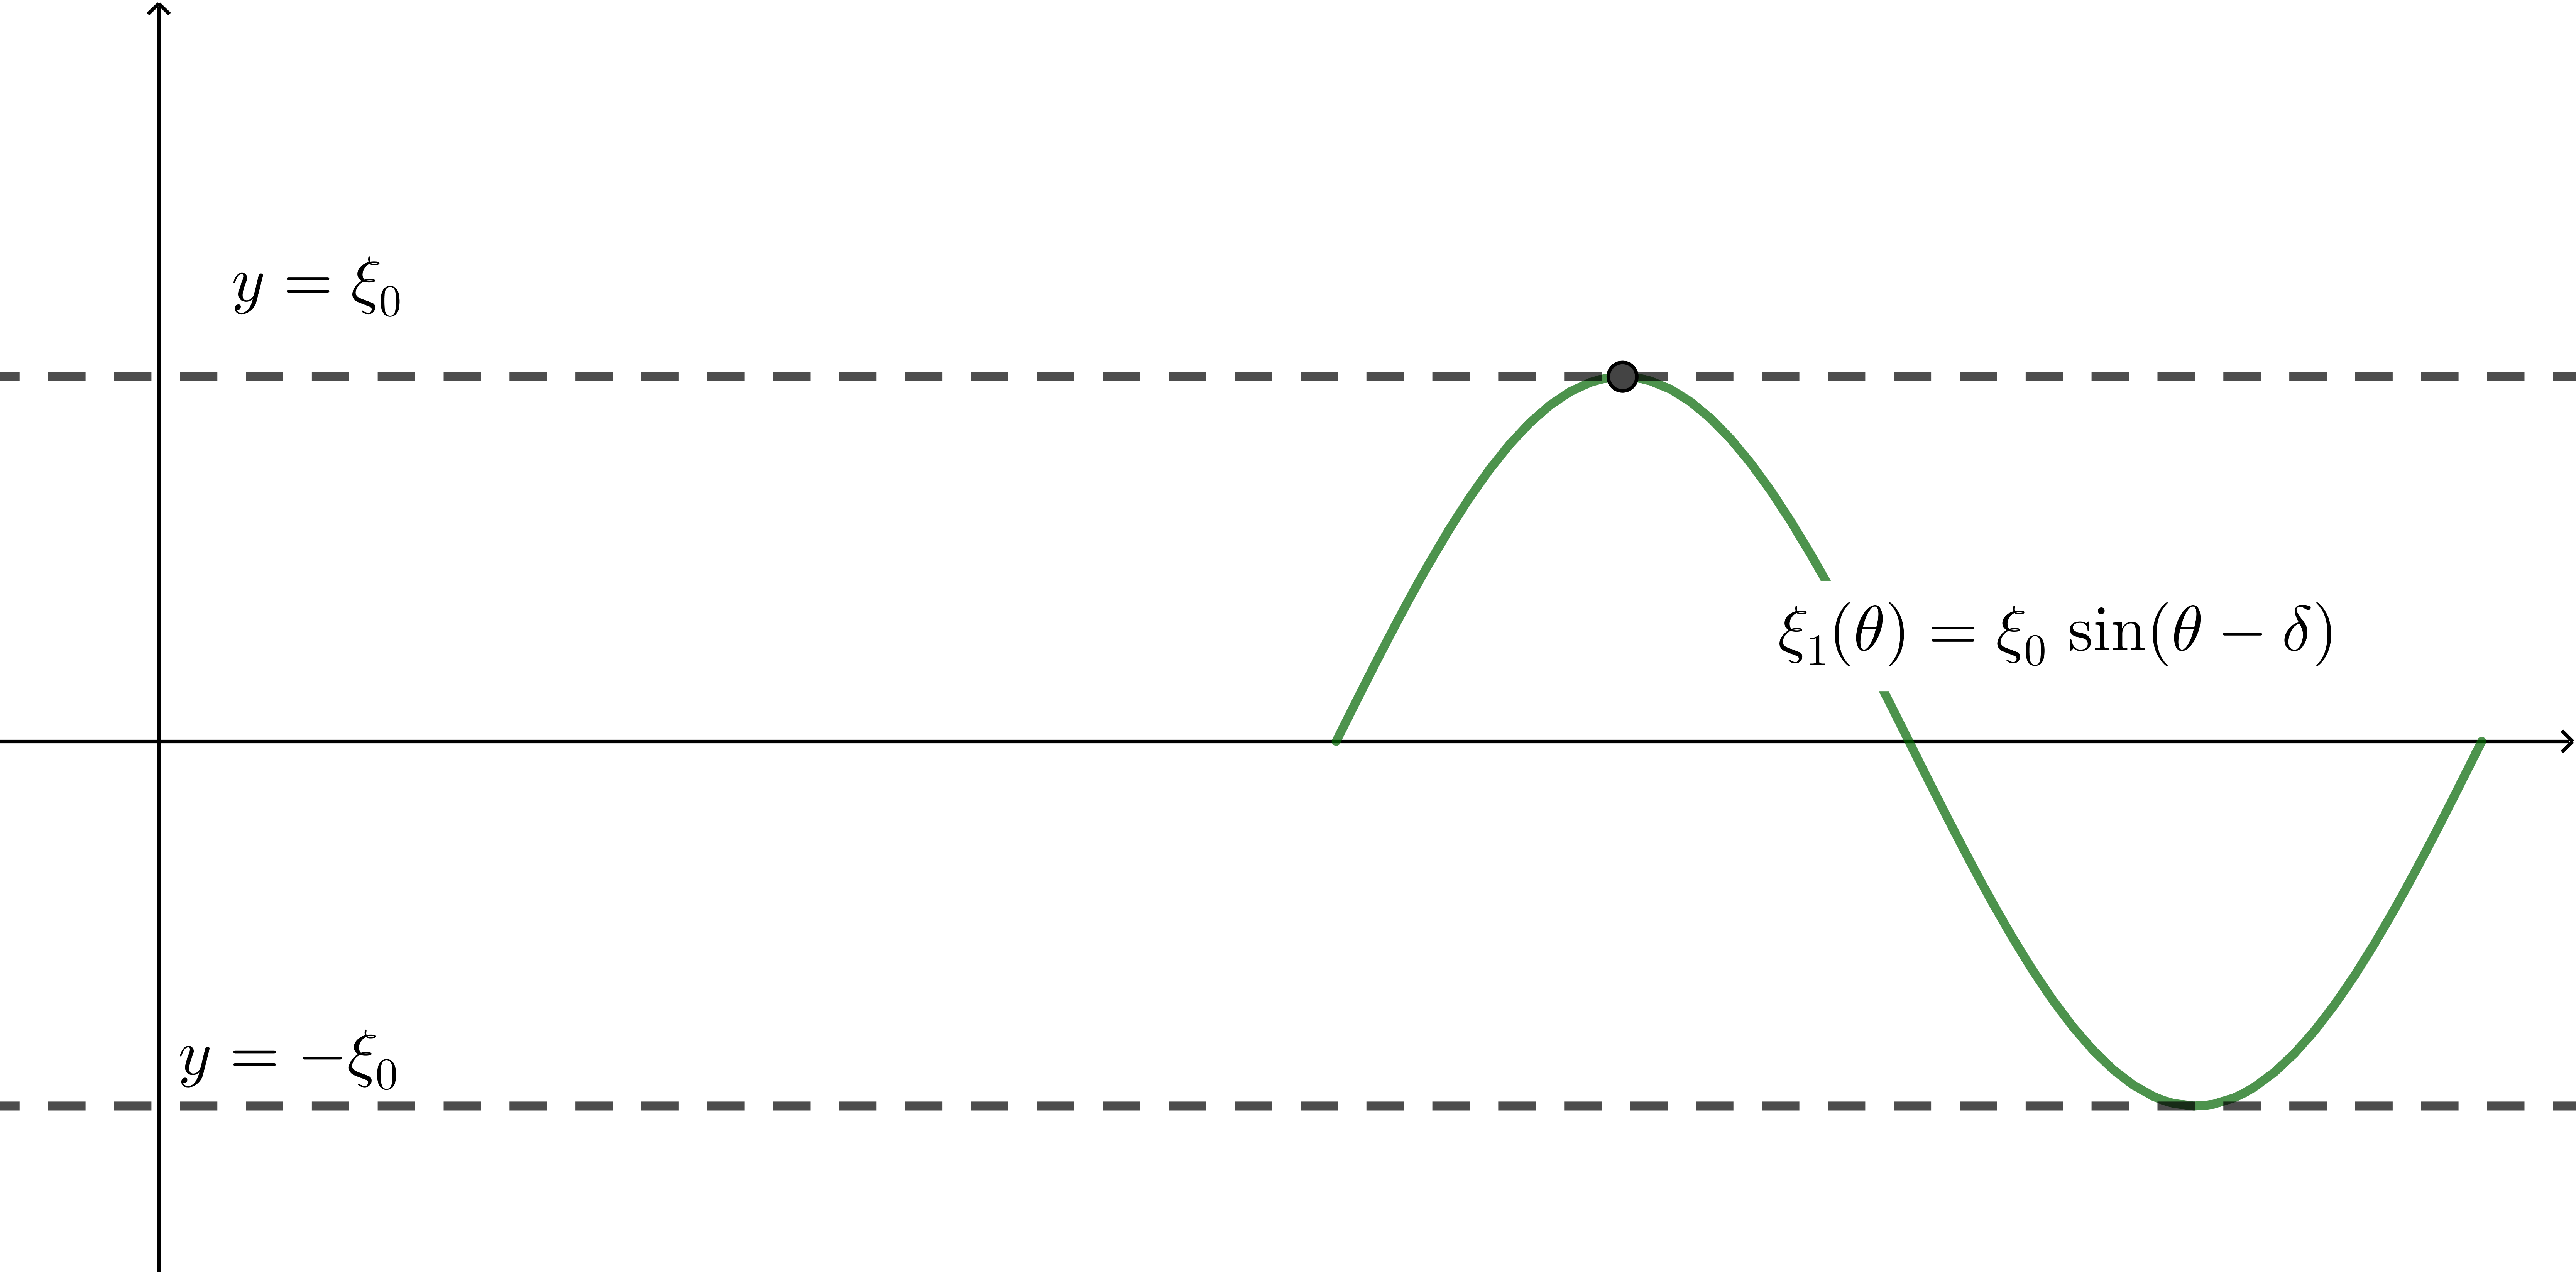
\includegraphics[width=0.7\linewidth]{geogebra-seno-2}
	\label{fig:geogebra-seno-2}
\end{figure}
Os dois gráficos anteriores, agora compartilhando do mesmo conjunto de eixos no desenho, como mostrado na figura \ref{fig:geogebra-seno-3}, permite-nos vislumbrar que ambos são semelhantes na forma, estão deslocados no espaço (eixo \( \theta \)) de uma distância igual a \( \delta \).
\begin{figure}[ht]
	\centering
	\caption[]{Confrontação dos gráficos de duas funções harmônica inter deslocadas.}
	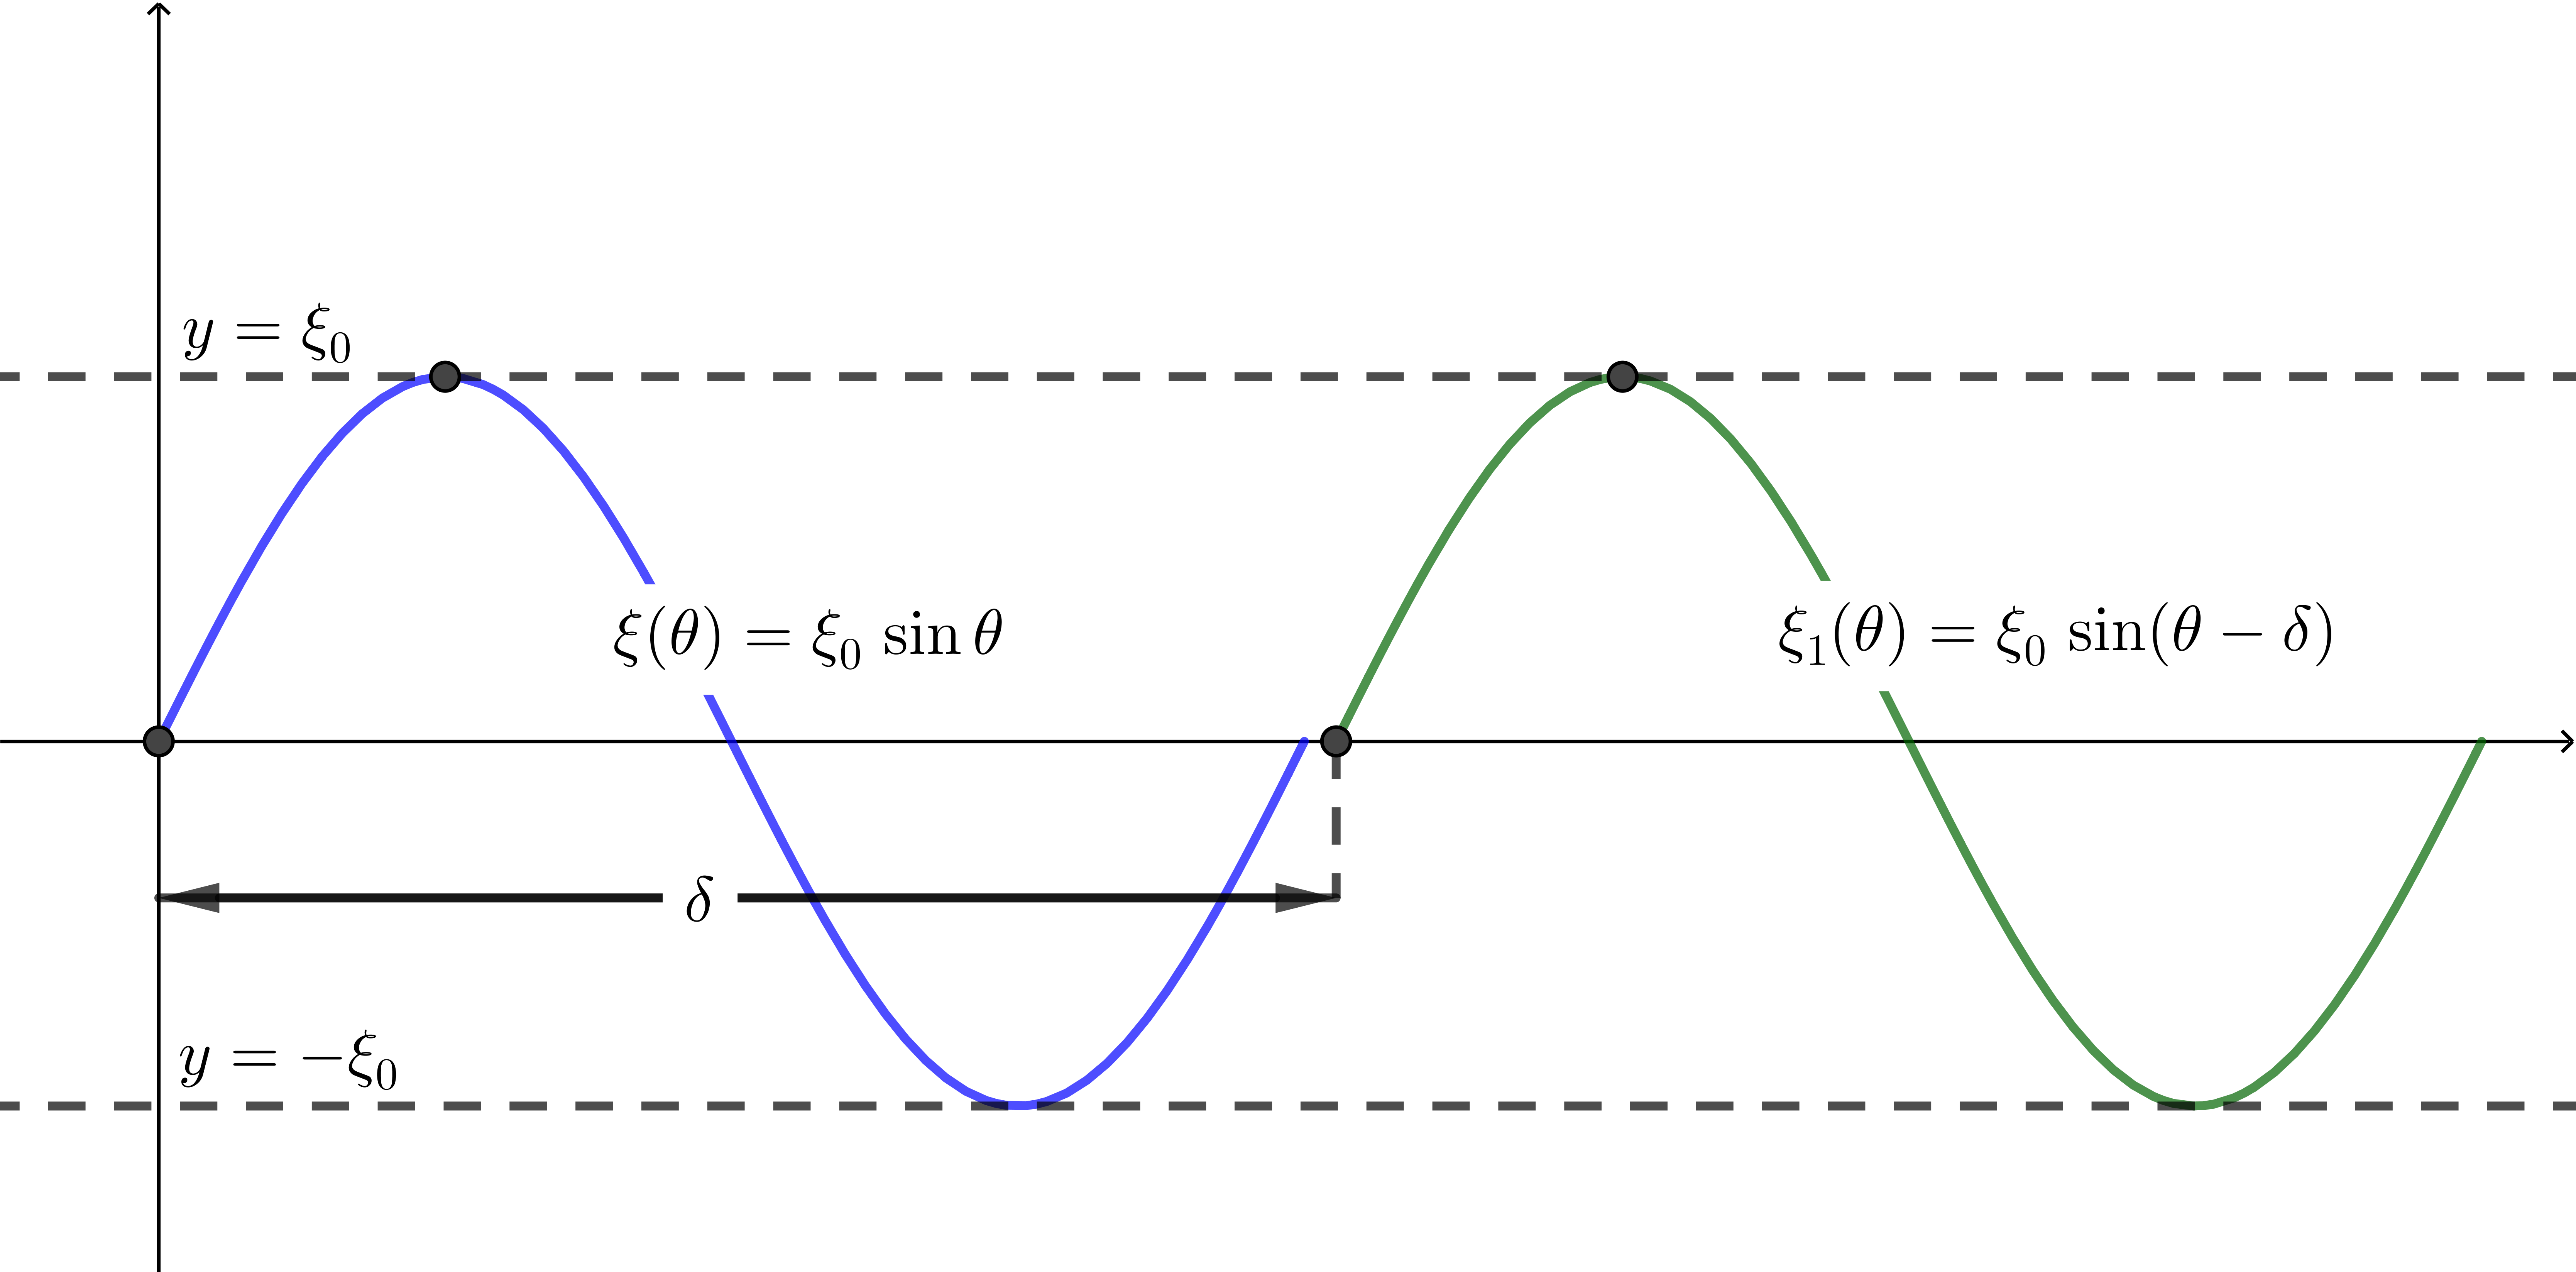
\includegraphics[width=0.7\linewidth]{geogebra-seno-3}
	\label{fig:geogebra-seno-3}
\end{figure}
Assim, diz-se que a função \( \xi_1 \) é uma translação de \( \xi \). Ressalte-se que estamos tratando com uma \emph{variável independente} que representa valores em radianos, qual seja, a variável  \( \theta \). Então daqui em diante temos que associar uma grandeza para melhor representar os sistemas físicos.
Podemos fazê-lo por meio da transformação matemática: \[ \theta = k\, x - \delta\text{,}\]onde a variável \( x \) estará com aí presente para representar de fato uma posição, agora, no eixo X. Isso nos permite propor as seguintes descrições físicas:
\begin{itemize}
	\item o traçado da senoide como que representando o efeito de uma onda tem origem na posição onde uma fonte impõe oscilação ou vibração ao meio.
	\item  a partir daí o meio absorve e ao mesmo tempo transmite a energia e quantidade de movimento para sua vizinhança também na forma de oscilações locais.
\end{itemize}

A presença de um fenômeno físico ondulatório, cujo perfil da onda estaria sendo esboçado pela senoide do lado direito da figura \ref{fig:geogebra-seno-3}, sugere que ele, o perfil, é uma repetição do que está à esquerda, ou seja, o perfil atual é uma repetição gráfica e manterá a sua extensão unidirecional medida em \emph{radianos}, durante as repetições sucessivas. Então, para um determinado valor de \( x \):
\begin{itemize}
	\item  é verdadeira a proposição,  \[\sin\qty(2\,\pi + k\,x - \delta) \,=\, \sin\qty(k\,x-\delta)\text{,}\] qualquer que seja o valor de \( x \).
	\item e, consequentemente, estender tal argumentação diretamente para a expressão do perfil de onda senoidal. 
\end{itemize}
De forma algébrica, temos:
\[ \xi \qty(x)\, =\, \xi_0 \sin \qty( k\, x - \delta)\]
ou 
\begin{equation}\label{eq-delta/k}
	\xi \qty(x)\, =\,  \xi_0 \sin k \qty(x- \frac{\delta}{k})\text{,}
\end{equation}
e da mesma forma
\[ \xi\qty(x)\,=\,\xi_0\sin k\qty(\frac{2\,\pi}{k}+ x- \frac{\delta}{k})\text{,} \]
%%%%%%%%%%%%%%%%%%%%%%%%%%%%


Se considerarmos neste momento, o \( k \) como um coeficiente contante, então a quantidade \(\frac{2\,\pi}{k}  \) também o será. Tal quantidade, a qual é do mesmo tipo de grandeza de \( x \), é denominada \emph{comprimento de onda} \( \lambda \)\footnote{Observar que essa quantidade corresponde à constante \(T\) apresentada no preâmbulo do capítulo \ref{estudos}, a qual caracteriza uma função periódica.}, ou seja, é o comprimento do perfil da onda ao longo do eixo X. Temos então,
\begin{equation*}\label{lambda}
	\lambda= \frac{2\,\pi}{k}\text{.}
\end{equation*}
Vamos a um exemplo prático representado no ambiente Maxima.

\noindent
% Code cell para função trigonométrica abordadem matemática
\begin{minipage}[t]{\textwidth}\color{blue}
	\centering
	\noindent
	\texttt{CODE CELL MAXIMA}
\end{minipage}
\rule{\linewidth}{.1em}


\noindent
%%%%%%%%
%% INPUT:
\begin{minipage}[t]{4.000000em}\color{red}\bfseries
	--\ensuremath{\ensuremath{>}}	
\end{minipage}
\begin{minipage}[t]{\textwidth}\color{blue}
	A:\ [\ensuremath{\xi}\_0:\ 7,\ k:\ 3,\ \ensuremath{\delta}\ :20]\ /*\ valores\ arbitrários.\ */\$\ \ensuremath{\lambda}:\ 2*\%pi/k\$\\
	\ensuremath{\xi}(x):=\ A[1]*\ sin(A[2]*(\ \ensuremath{\lambda}\ +\ x\ -\ A[3]/A[2]\ ))\$\ disp(\ `\ensuremath{\lambda}\ =\ \ensuremath{\lambda},\ \ensuremath{\xi}(x)\ =\ \ensuremath{\xi}(x))\$\\
	wxplot2d([\ensuremath{\xi}(x)],\ [x,0,\ x\_1:\ 6],\ [style,\ lines],\ [color,\ brown],\ nobox\ )\$
\end{minipage}

\noindent%


\begin{figure}[H]
	\centering
	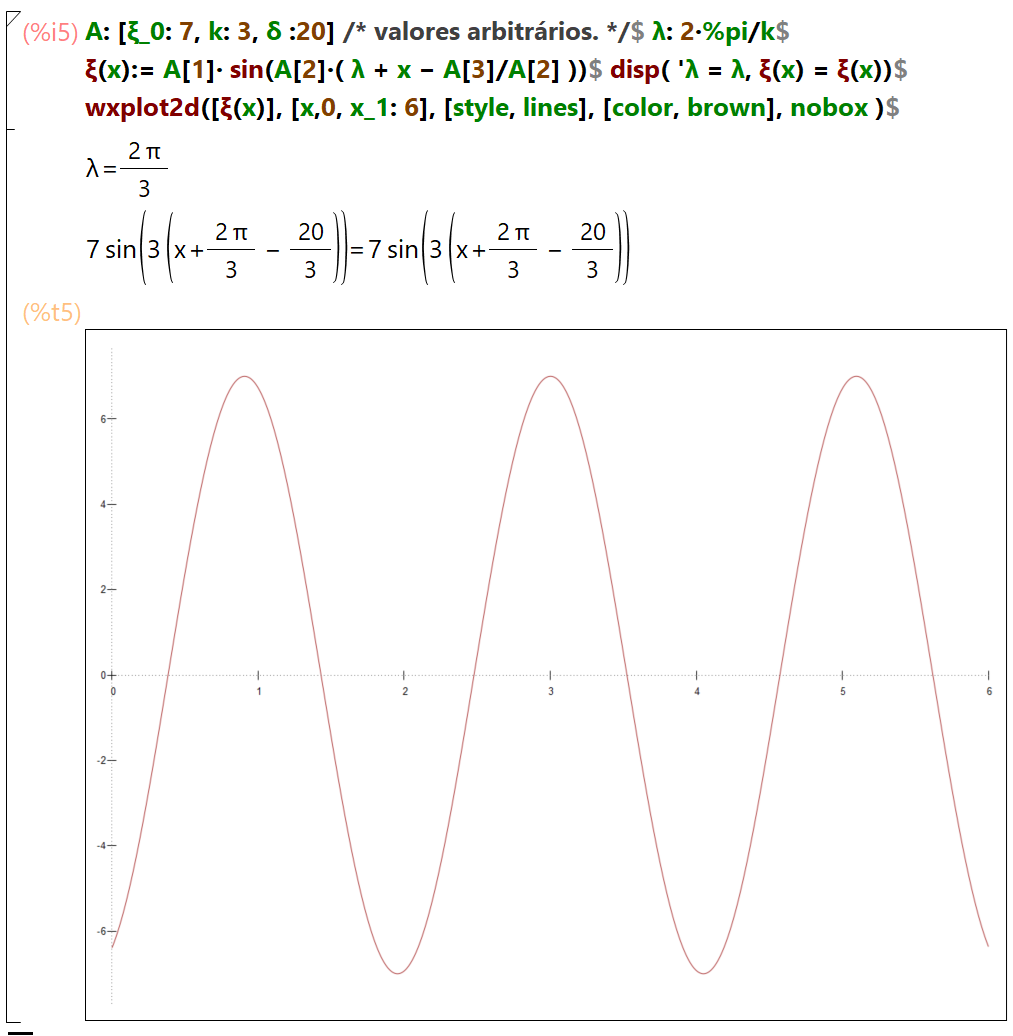
\includegraphics[width=0.8\linewidth]{conprimentoDeOnda}
	%\caption{}
	\label{fig:conprimentodeonda}
\end{figure}

\noindent
% Code cell para função trigonométrica abordadem matemática
\begin{minipage}[t]{\textwidth}\color{blue}
	\centering
	\noindent
	\texttt{CODE CELL MAXIMA}
\end{minipage}
\rule{\linewidth}{.1em}
\noindent
\begin{minipage}[t]{4.000000em}\color{red}\bfseries
	--\ensuremath{\ensuremath{>}}	
\end{minipage}
\begin{minipage}[t]{\textwidth}\color{blue}
	A:\ [\ensuremath{\xi}\_0:\ 7,\ k:\ 3,\ \ensuremath{\delta}\ :20]\ /*\ valores\ arbitrários.\ */\$\ \ensuremath{\lambda}:\ 2*\%pi/k\$\\
	\ensuremath{\xi}(x):=\ A[1]*\ sin(A[2]*(\ \ensuremath{\lambda}\ +\ x\ -\ A[3]/A[2]\ ))\$\ disp(\ '\ensuremath{\lambda}\ =\ \ensuremath{\lambda},\ '\ensuremath{\xi}(x)\ =\ \ensuremath{\xi}(x))\$\\
	/*\ Conjunto\ de\ pontos.\ */\ \ensuremath{\xi}:\ makelist([x,\ensuremath{\xi}(x)],x,0,x\_1:\ 6,0.05)\$\\
	wxplot2d([discrete,\ \ensuremath{\xi}],\ [style,\ points],\ [color,\ blue],\ [point\_type,\ asterisk])\$
\end{minipage}

\noindent%

\begin{figure}[H]
	\centering
	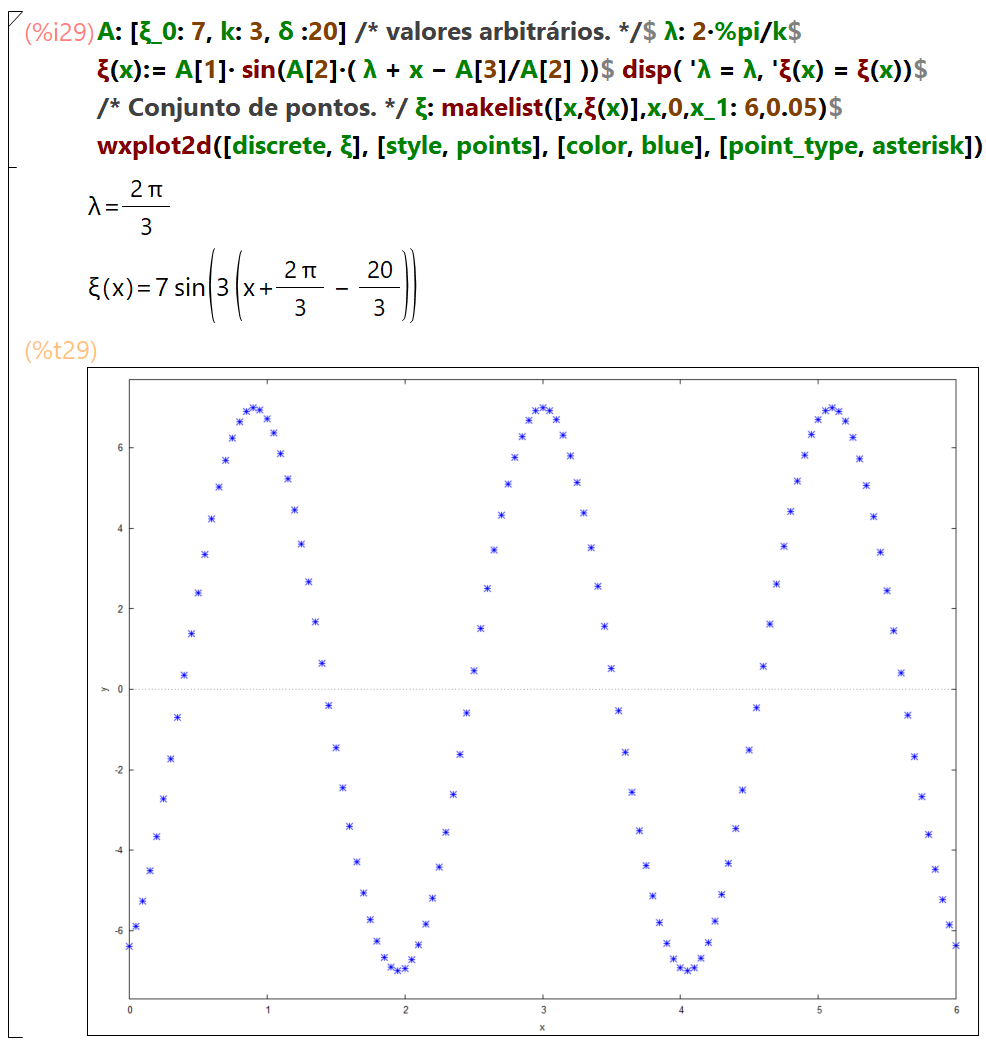
\includegraphics[width=.85\linewidth]{conprimentoDeOnda1}
	%\caption{}
	\label{fig:conprimentodeonda1}
\end{figure}

% Code cell para função trigonométrica abordadem matemática
\begin{minipage}[t]{\textwidth}\color{blue}
	\centering
	\noindent
	\texttt{CODE CELL MAXIMA}
\end{minipage}
\rule{\linewidth}{.1em}
\noindent


\noindent
%%%%%%%%
%% INPUT:
\begin{minipage}[t]{4.000000em}\color{red}\bfseries
	--\ensuremath{\ensuremath{>}}	
\end{minipage}
\begin{minipage}[t]{\textwidth}\color{blue}
	A:\ [\ensuremath{\xi}\_0:\ 7,\ k:\ 3,\ \ensuremath{\delta}\ :20]\ /*\ valores\ arbitrários.\ */\$\ \ensuremath{\lambda}:\ 2*\%pi/k\$\\
	\ensuremath{\xi}(x):=\ A[1]*\ sin(A[2]*(\ \ensuremath{\lambda}\ +\ x\ -\ A[3]/A[2]\ ))\$\ disp(\ '\ensuremath{\lambda}\ =\ \ensuremath{\lambda},\ '\ensuremath{\xi}(x)\ =\ \ensuremath{\xi}(x))\$\\
	/*\ Pontos.\ */\ \ensuremath{\xi}:\ makelist([x,\ensuremath{\xi}(x)],x,0,x\_1:\ 6,0.05)\$\\
	/*\ pacote\ "draw".\ */\ wxdraw2d\\
	(point\_type\ =\ filled\_circle,\ point\_size\ \ \ \ =2,\ color\ =\ red,\ points(\ensuremath{\xi})\ )\$
\end{minipage}

\noindent%

\begin{figure}[H]
	\centering
	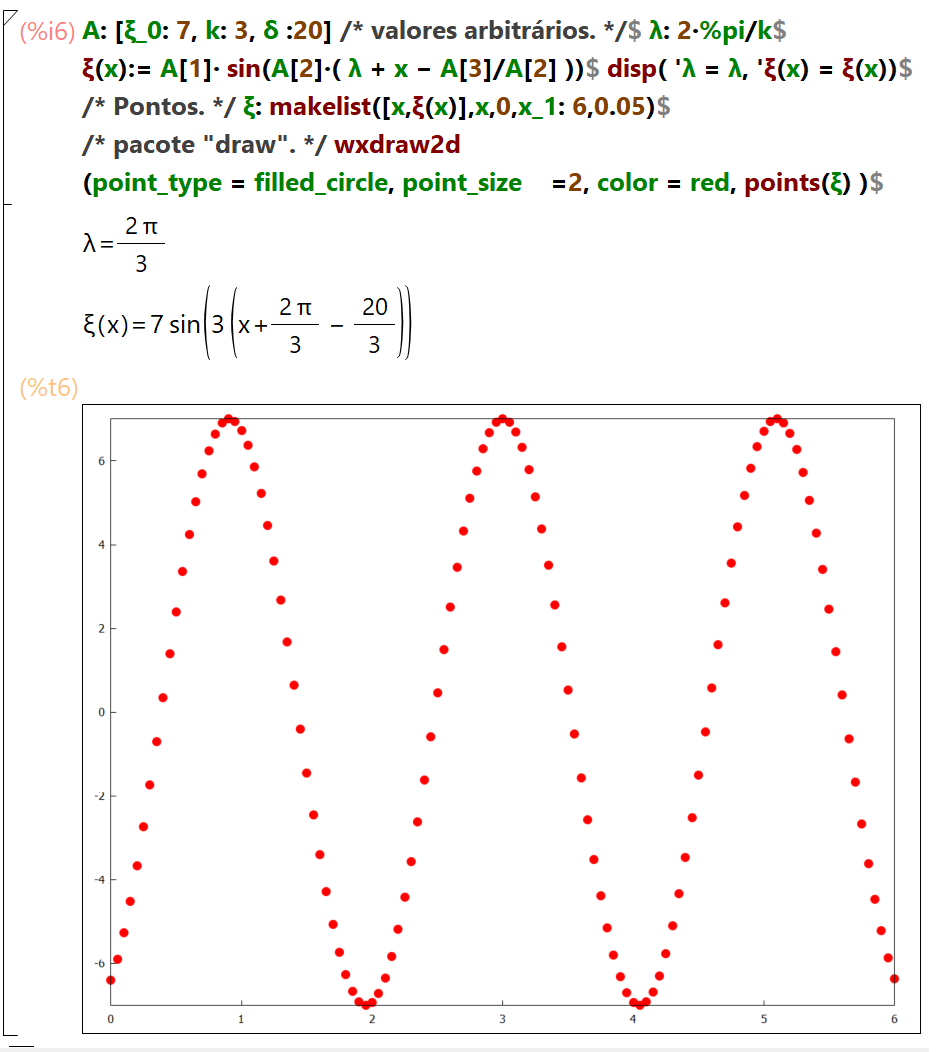
\includegraphics[width=0.8\linewidth]{conprimentoDeOnda2}
	%\caption{}
	\label{fig:conprimentodeonda2}
\end{figure}


\section{Onda Harmônica como um Modelo Físico}
Até aqui trabalhamos com desenhos hipotéticos, mas, numa situação real, uma onda o é de fato assim considerada se observadas as características que confirmam sua presença no meio. Uma dessas é o movimento de vai e vem dos elementos que constituem o meio que está sob efeito da suposta onda. Tal movimento é transferido sucessivamente de um ponto para sua vizinhança a cada momento.

Para refletir essa condição há de se fazer o perfil, ora representado por uma senoide, como algo em movimento ou caminhante. Assim, a parcela \( \frac{\delta}{k} \) na equação \ref{eq-delta/k} passa a ser escrita com a  conotação de tempo por meio do produto \( v\, t \),
\[ \frac{\delta}{k}\equiv v\, t \]
onde
\begin{enumerate}
	\item  \( t \) é a variável independente tempo;
	\item  \( v \) é a velocidade com que o perfil estaria se movimentando,  é chamada \emph{velocidade de fase}. No caso da onda harmônica seu perfil não altera, portanto todas as fases da onda caminham à mesma velocidade.
\end{enumerate}
%\[ \xi\qty(x,t) = \xi_0\, \sin \qty(k\,x-v\,t)\text{,}\]
Reescrevendo a equação \ref{eq-delta/k}, nesses termos,
\[ \xi\qty(x,t) = \xi_0\, \sin k \qty(x-v\, t)\text{,}\]
e, fazendo \( k= \frac{2\, \pi}{\lambda} \), temos
\[ \xi\qty(x,t) = \xi_0\, \sin \qty(k\, x - \frac{2\,\pi}{\lambda}\,v\,t)\text{,}\]
que reescrevendo fica,	
\[ \xi\qty(x,t) \,=\, \xi_0\,  \sin \qty(k\, x - \frac{2\,\pi}{\frac{\lambda}{v}}\,t)\text{.}  \]
O termo \(  \nicefrac{\lambda}{v} \) é denominado \emph{período de oscilação}, \( P \),  em cada ponto \( x \) sujeito ao efeito da onda (os vai e vens), é expresso em unidades de tempo. Consequentemente define-se a \emph{frequência angular} da onda, \( \omega \), em radianos por unidade de tempo
\begin{equation}\label{freqAngular}
	\omega\, =\, \frac{2\, \pi}{P}\text{.}
\end{equation}
Portanto, escreve-se, para um onda harmônica, movendo-se (propagando-se) para o sentido positivo do eixo X,
\begin{equation}\label{harmonica}
	\xi\qty(x,t) = \xi_0 \sin\qty(k\,x - \omega\,t)\text{.}
\end{equation}
Uma vez que ciclo de oscilação possui \( 2\, \pi\, \mathrm{rad}\), podemos definir uma grandeza $\nu$ por meio da expressão,
\begin{equation}\label{frequencia}
	\nu = \frac{\omega}{ 2\,\pi}\text{,}
\end{equation}
que corresponderá à taxa em \emph{ciclos (ou fração de ciclo) por unidade de tempo} com que oscilações (efeito local da onda) estão perpassando no ponto $x$.
A partir da equação \ref{frequencia}, podemos fazer \( \omega= 2\, \pi\, \nu \) e comparar com o segundo membro da equação \ref{freqAngular}, do que se deduz \( P = \frac{1}{\nu} \). Asim temos,
\[ P= \frac{\lambda}{v} = \frac{1}{\nu}\text{,} \]
de onde se deduz 
\begin{equation}\label{lambdaFundamental}
	\lambda\, \nu = v \text{,}
\end{equation}
e, também a equação
\begin{equation}\label{lambda-2}
	\lambda = v\, P\text{,}
\end{equation}
a qual permite a interpretação de \( \lambda \) como a distância que é percorrida pelo movimento ondulatório ao tempo de um período, \( P \).
Uma vez que apliquemos \( x=0 \) na equação \ref{harmonica}, resulta \( \xi \qty(0,t) = \xi_0 \sin\qty( - \omega\,t) \). Se a fonte da oscilação estiver a começar a atuar nessa posição, ou seja, \( t=0 \), então teremos \( \xi \qty(0,0) = 0\).
O valor de \( \xi  \), em \( t=0 \) chama-se \emph{condição inicial} e, não necessariamente, terá o valor sempre igual a zero. Por conta disso podemos escrever tal quantidade na forma literal, \(  \xi\qty(0,0)=\xi_0\, \sin\phi  \).  Assim a equação  \ref{harmonica} passa a ser escrita de forma mais geral como:
\begin{equation}\label{phi}
	\xi\qty(x,t) = \xi_0 \sin\qty(k\,x - \omega\,t+\phi)\text{,}
\end{equation}
onde \( \phi \) é medida em radianos e chamada \emph{constante de fase}. A presença dessa contante de fase não altera a forma da onda, apenas a desloca sobre o eixo X ou no eixo dos tempos.
O valor \( k \) mencionado inicialmente possui um significado importante, ele é o \emph{número de onda}. A partir da equação \ref{lambda} podemos fazer \( k\,\lambda= 2\,\pi \), de onde se tira que \( k \) indica quantos comprimentos de onda então contidos na distância \( 2\, \pi \) radianos.\\


%{ {\scshape Exemplo \thesection.\theexemplos:}} 
Seja uma função senoidal \( y= 5\,\sin x -2 \), que representa uma grandeza a qual iniciou um movimento ondulatório na direção positiva do eixo X. A velocidade angular foi determinada no valor de dois radiano por segundo. Vamos representar essa condição no wxMaxima.

\noindent
% Code cell para onda caminhante - exemplo
\begin{minipage}[t]{\textwidth}\color{blue}
	\centering
	\noindent
	\texttt{CODE CELL MAXIMA}
\end{minipage}
	\rule{\linewidth}{.1em}
\noindent
\begin{minipage}[t]{4.000000em}\color{red}\bfseries
	--\ensuremath{\ensuremath{>}}	
\end{minipage}
\begin{minipage}[t]{\textwidth}\color{blue}
	A:\ [\ \ensuremath{\xi}\_0:\ 5,\ k:\ 1,\ \ensuremath{\omega}:\ 2\ ,\ \ensuremath{\phi}:\ 2\ ]\ /*\ parâmetros\ do\ movimento\ ondulatório\ em\ t=0.\ \ */\$\\
	\ensuremath{\xi}(x,\ t):=\ A[1]*sin(\ A[2]*x\ -A[3]*t\ +A[4]\ )\$\\
	print("Onda\ caminhante:\ ",\ \ "\ensuremath{\xi}(x,\ t)\ =",\ \ensuremath{\xi}(x,\ t)\ \ )\$
\end{minipage}

\noindent%

\begin{figure}[H]
	\centering
	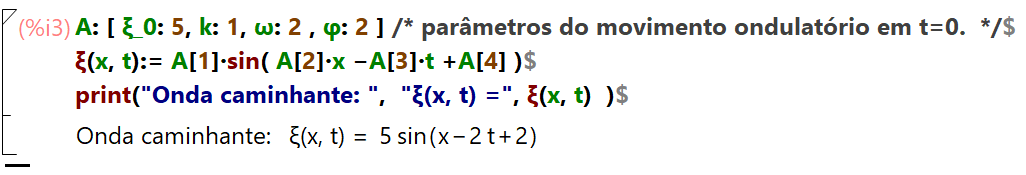
\includegraphics[width=1\linewidth]{ondaCaminhante}
	%\caption{}
	\label{fig:ondacaminhante}
\end{figure}

%\newpage
%\setcounter{exemplos}{2}
%{ {\scshape Exemplo \thesection.\theexemplos:}} 
\newpage
Supondo que a fonte de oscilação do exemplo anterior manteve-se continuamente em ação \footnote{Neste caso, disse-se que há um \emph{trem de ondas}.}. E em algum momento ocorreu um processo sobre movimento que `deslocou' a onda para frente. De tal forma que no ponto de fase igual a \(\frac{3\, \pi}{2}\,\mathrm{rad} \) a amplitude passou a ser \(80\%\) do valor original. Vamos analisar tal condição no wxMaxima.

\noindent
% Code cell para onda caminhante - exemplo
\begin{minipage}[t]{\textwidth}\color{blue}
	\centering
	\noindent
	\texttt{CODE CELL MAXIMA}
\end{minipage}
	\rule{\linewidth}{.1em}
\noindent
%%%%%%%%
%% INPUT:
\begin{minipage}[t]{4.000000em}\color{red}\bfseries
	--\ensuremath{\ensuremath{>}}	
\end{minipage}
\begin{minipage}[t]{\textwidth}\color{blue}
	kill(all)\$\ A:\ [\ \ensuremath{\xi}\_0:\ 5,\ k:\ 1,\ \ensuremath{\omega}:\ 2\ ,\ $\phi$:\ 2\ ]\ /*\ parâmetros\ do\ movimento\ em\ t=0.\ */\$\\
	numer:\ true\$\ fpprintprec:\ 3\$\ \ensuremath{\xi}(x,\ t):=\ A[1]*sin(\ A[2]*x\ -A[3]*t\ +A[4])\$\\
	/*\ Fase\ inicial.*/\ \ \ensuremath{\theta}:\ 3*\%pi/2\$\ /*\ \ \ensuremath{\Delta}\ensuremath{\delta},\ deslocamento\ da\ fase.\ */\\
	/*\ Equação\ de\ balanço.*/\ \ EQ:\ A[1]*\ sin(\ensuremath{\theta}+\ensuremath{\Delta}\ensuremath{\delta})\ =\ \ 0.5\ *A[1]*\ sin(\ensuremath{\theta})\$\\
	SOL:\ rat(solve(EQ,\ \ensuremath{\Delta}\ensuremath{\delta}))\$\ /*\ SOL\ retorna\ como\ lista.\ */\\
	\ensuremath{\Delta}\ensuremath{\delta}:\ float(pickapart(part(SOL[1],2),3))\$\ /*\ retorna\ apenas\ o\ valor.\ \ */\\
	print($\blacktriangleleft$
	"\ Onda\ inicial:\ ",\ "\ensuremath{\xi}(x,\ t)\ =",\ \ensuremath{\xi}(x,\ t)\ )\$\\
	\ensuremath{\xi}\_1(x,\ t):=\ A[1]*sin(\ A[2]*x\ -A[3]*t\ +(A[4]+\ensuremath{\Delta}\ensuremath{\delta})\ )\$\\
	print($\blacktriangleleft$
	"\ Onda\ final:\ ",\ "\ensuremath{\xi}(x,\ t)\ =",\ \ensuremath{\xi}\_1(x,\ t)\ )\$\\
	/*\ Plotagem.\ */\ H(x)\ :=\ if\ x\ \ensuremath{<}\ (3*\%pi/2\ -\ 2)\ then\ \ensuremath{\xi}(x,\ 0)\ else\ \ensuremath{\xi}\_1(x,\ 0)\$\\
	wxplot2d(\ \ H(x),\ [x,-10,10]\ ,\ nobox\ \ )\$
\end{minipage}

\noindent%
\begin{figure}[H]
	\centering
	\includegraphics[width=0.75\linewidth]{modeloFísico}
	%\caption{}
	\label{fig:modelofisico}
\end{figure}
\newpage
%\setcounter{exemplos}{3}
%{ {\scshape Exemplo \thesection.\theexemplos:}} 
Um determinado movimento ondulatório arbitrário tem como função de onda a expressão dada por
\[\xi\qty(x,t)= \sqrt2\sin\qty(2\,x-t)\text{,}\] 
vamos analisar a posição do ponto em \(x=2\) para quatro momentos de tempo diferentes e arbitrários.

\noindent
% Code cell para onda caminhante - exemplo
\begin{minipage}[t]{\textwidth}\color{blue}
	\centering
	\noindent
	\texttt{CODE CELL MAXIMA}
\end{minipage}
\rule{\linewidth}{.1em}
\noindent
\begin{minipage}[t]{4.000000em}\color{red}\bfseries
	--\ensuremath{\ensuremath{>}}	
\end{minipage}
\begin{minipage}[t]{\textwidth}\color{blue}
	kill(all)\$declare\_subscripted(\ensuremath{\xi}\_0)\$\ \ensuremath{\xi}\_0:\ sqrt(2)\$\\
	t:\ [t\_1:\ 0.5,\ t\_2:\ 1,\ t\_3:\ 5,\ t\_4:\ 5.5]\$\ \ensuremath{\xi}[i](x):=\ \ensuremath{\xi}\_0*sin(\ \ 4*x/3\ -\ t[i]\ )\ \$\\
	set\_draw\_defaults(\ axis\_top=false,\ axis\_bottom=false,\ axis\_right\ =\ false,\ xtics\_axis=true,\ \\
	\ \ \ \ xrange\ =\ [0,4],\ yrange\ =\ [-1.7,1.7],\ \ \ point\_type\ =\ \ensuremath{\sim\ }filled\_circle,\ point\_size\ =\ensuremath{\sim\ }0\ ,\ \\
	\ \ \ \ ip\_grid\_in=[1,1],\ \ ip\_grid=[1,1],\ \ grid\ \ \ =\ true,\ \ title\ \ =\ "Plotagem\ tempo\ a\ tempo"\ )\$\\
	wxdraw2d(color=blue,\\
	\ \ \ \ explicit(\ensuremath{\xi}[1],x,0,4),\ \ \ points(\ \ \ [2,\ensuremath{\xi}[1](2)]\ \ )\ \ ,\ label(\ [concat("t\_1=\ ",\ t[1]),\ 2,\ensuremath{\xi}[1](2)\ ]\ ),\\
	\ \ \ \ explicit(\ensuremath{\xi}[2],x,0,4),\ \ \ points(\ \ \ [2,\ensuremath{\xi}[2](2)]\ \ )\ \ ,\ label(\ [concat("t\_2=\ ",\ t[2]),\ 2,\ensuremath{\xi}[2](2)\ ]\ ),\\
	\ \ \ \ explicit(\ensuremath{\xi}[3],x,0,4),\ \ \ points(\ \ \ [2,\ensuremath{\xi}[3](2)]\ \ )\ \ ,\ label(\ [concat("t\_3=\ ",\ t[3]),\ 2,\ensuremath{\xi}[3](2)\ ]\ ),\\
	\ \ \ \ explicit(\ensuremath{\xi}[4],x,0,4),\ \ \ points(\ \ \ [2,\ensuremath{\xi}[4](2)]\ \ )\ \ ,\ label(\ [concat("t\_4=\ ",\ t[4]),\ 2,\ensuremath{\xi}[4](2)\ ]\ )\ \ )\$
\end{minipage}
\noindent%
\begin{figure}[H]
	\centering
	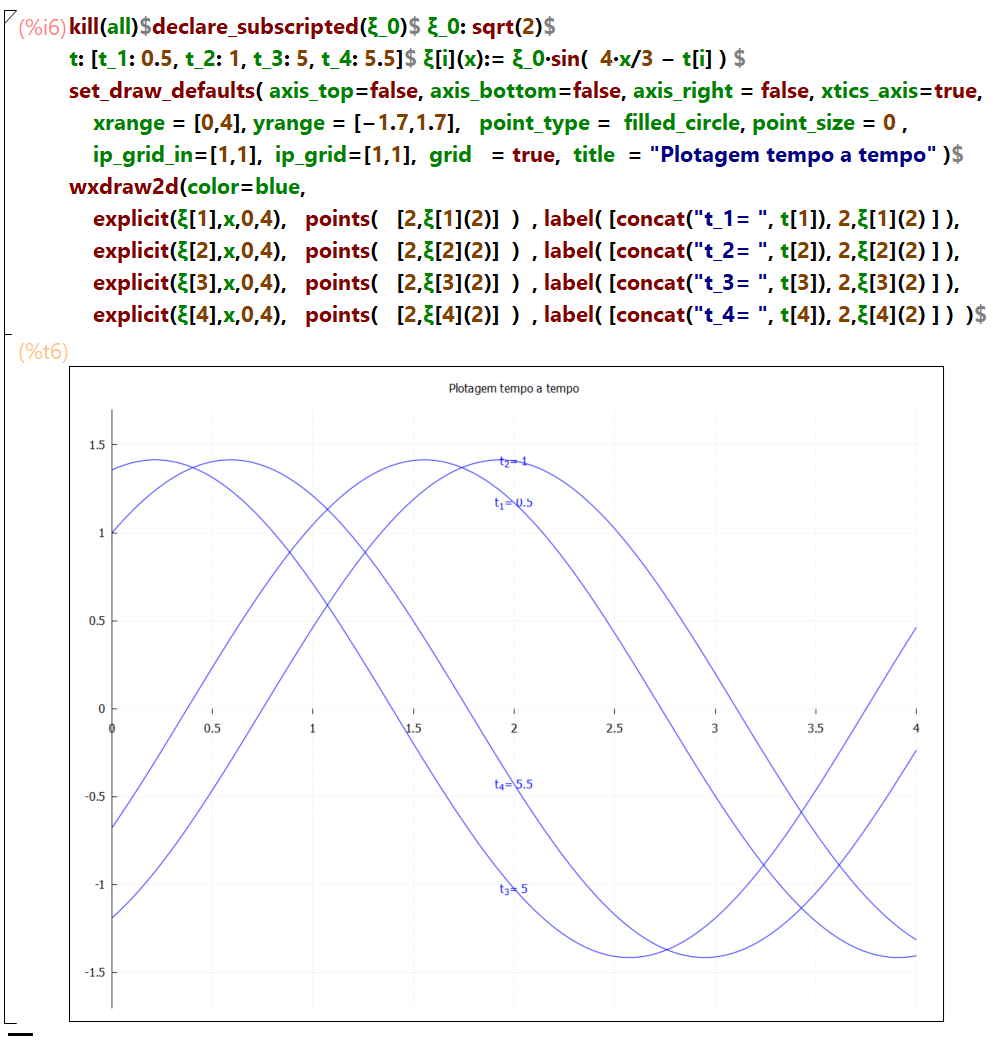
\includegraphics[width=0.75\linewidth]{conprimentoDeOnda3}
	%\caption{}
	\label{fig:conprimentodeonda3}
\end{figure}
\newpage
Duas ondas propagam-se em uma mesma direção ao longo de uma dimensão retilínea de um meio perfeitamente elástico e acontece interferência. Supondo elas estando com um mesmo comprimento de onda e mesma velocidade de propagação. A amplitude de cada onda é de \( 9,7 \mathrm{mm}\) e há uma diferença de fase de \(110\degree\). Vamos analisar essa interferência no Maxima.

\noindent
% Code cell para onda caminhante - exemplo
\begin{minipage}[t]{\textwidth}\color{blue}
	\centering
	\noindent
	\texttt{CODE CELL MAXIMA}
\end{minipage}
\rule{\linewidth}{.1em}
\noindent
\begin{minipage}[t]{4.000000em}\color{red}\bfseries
	--\ensuremath{\ensuremath{>}}	
\end{minipage}
\begin{minipage}[t]{\textwidth}\color{blue}
	load("trigtools"\ )\ \$\ fpprintprec\ :\ 3\$\\
	A:[\ k:1,\ \ensuremath{\omega}:\ 1,\ \ensuremath{\phi}\_1:\ 0,\ \ensuremath{\phi}\_2:\ 110\ ,\ \ensuremath{\xi}\_1:\ 9.7\ ,\ \ /*\ para\ k\ e\ \ensuremath{\omega}\ aqui\ os\ valores\ são\ hipotéticos.\ */\ \ \\
	\ \ \ \ \ \ensuremath{\xi}\_2:\ 9.7\ ]\$\ \ \\
	A:\ append(\ \ \ A,\ [A[3]*\%pi/180,\ A[4]*\%pi/180]\ \ \ \ )\$\\
	/*\ Ondas\ superpostas.\ */\ \ensuremath{\xi}(x,t):=\ [\ A[5]*\ sin(\ A[1]*x\ -\ A[2]*\ t\ -A[7]\ ),\ \\
	\ \ \ \ A[6]*\ sin(\ \ A[1]*x\ -\ A[2]*\ t\ -\ A[8]),\\
	/*Onda\ resultante.*/\ A[5]*\ sin(\ A[1]*x\ -\ A[2]*\ t\ -A[7]\ )\ +A[6]*\ sin(\ \ A[1]*x\ -\ A[2]*\ t\ -\ A[8])\ ]\$\\
	/*\ Amplitude.\ */\ \ \ \ensuremath{\xi}\_3:\ float(\ sqrt(\ \ A[5]\verb|^|\ 2\ +\ A[6]\verb|^|\ 2\ +\ 2*\ A[5]*A[6]*cos(A[8]-A[7])\ ));\\
	numer:false\$\\
	/*\ Solução\ no\ ponto\ de\ máximo\ */\ sol:\ \ float\ (\ trigsolve\ (\ float(\ \ensuremath{\xi}(x,0)[3])=\ensuremath{\xi}\_3\ ,\ 2,3\ \ \ \ )\ );\ \\
	x\_max:\ first(sol);\\
	wxdraw2d(grid\ \ =\ true,\ xtics\_axis\ =\ true,\ xaxis\ =\ true,\ axis\_top=false,\ axis\_right=false,\\
	\ \ \ \ axis\_bottom\ =\ false,\ explicit(\ \ensuremath{\xi}(x,0)[1],\ \ x,0,4*\%pi),\ \ explicit(\ \ \ensuremath{\xi}(x,0)[2],\ \ x,0,4*\%pi),\\
	\ \ \ \ line\_width=5,\ color=red,\ \ line\_type\ =\ solid,\ \ explicit(\ \ensuremath{\xi}(x,0)[3],\ \ x,0,4*\%pi),\ \\
	\ \ \ \ point\_type\ =\ filled\_circle,\ point\_size\ =\ 2,\ points\_joined\ =\ false,\ color=blue,\\
	\ \ \ \ points(\ [\ [\ x\_max,\ 0],\ [x\_max,\ \ensuremath{\xi}\_3]\ ])\ ,font\_size\ =\ 20,\ font\ \ \ \ \ \ =\ "Arial",\\
	\ \ \ \ label(\ ["amplitude\ \ensuremath{\xi}\_3\ ",\ \ \ \ x\_max+1,\ \ensuremath{\xi}\_3\ ]\ \ \ ),\ label(\ ["x\_{max}\ ",\ \ \ \ x\_max+.5,\ 0\ ]\ )\\
	)\$
\end{minipage}
\noindent%
\begin{figure}[hp]
	\centering
	\includegraphics[width=.9\linewidth]{interferência}
	%\caption{}
	\label{fig:interferencia}
\end{figure}
\newpage
Ondas estacionárias podem ser produzidas em uma corda usando um gerador de pulsos mecânicos com determinada frequência. Vamos supor um tal mecanismo onde os ajustes sejam dados pela tração fornecida por uma massa dependurada em uma extremidade e na outra um motor fornece o movimento oscilatório. 

\noindent
% Code cell para onda caminhante - exemplo
\begin{minipage}[t]{\textwidth}\color{blue}
	\centering
	\noindent
	\texttt{CODE CELL MAXIMA}
\end{minipage}
\rule{\linewidth}{.1em}
\noindent
\begin{minipage}[t]{4.000000em}\color{red}\bfseries
	--\ensuremath{\ensuremath{>}}	
\end{minipage}
\begin{minipage}[t]{\textwidth}\color{blue}
	A:\ [/*Frequência\ do\ motor*/\ \ensuremath{\nu}:\ 120,\ /*Comprimento\ da\ corda.*/\ L:\ 1.2,\\
	\ \ \ \ /*massa\ específica.*/\ \ensuremath{\mu}:\ 1.6,\ \ /*padrão\ de\ movimento.*/\ n:\ 4,\ \ensuremath{\xi}\_0:\ 1\ /*(arbitrário).*/]\\
	\$fpprintprec:4\$\ /*velocidade\ angular*/\ensuremath{\omega}:\ float(2*\%pi*A[1])\$\\
	/*comprimento\ de\ onda*/\ \ensuremath{\lambda}\_n:\ 2*\ A[2]/A[4]\$\ /*número\ de\ onda*/\ k:\ float(2*\%pi/\ensuremath{\lambda}\_n)\$\\
	/*frequência\ estacionária.*/\ensuremath{\nu}\_n:\ \ \ A[1]\$\ /*velocidade\ de\ onda*/\ v:\ \ensuremath{\lambda}\_n\ *\ \ensuremath{\nu}\_n\$\ \\
	/*Amplitude\ da\ onda\ incidente.*/\ \$\ display([\ensuremath{\nu},\ L,\ \ensuremath{\mu},\ \ \ensuremath{\omega},\ \ensuremath{\lambda}\_n,\ k,\ v,\ \ensuremath{\nu}\_n,\ \ensuremath{\xi}\_0\ ]\ )\$\\
	/*amplitudes.*/A[5]:\ 2*A[5]\$\ \ \ensuremath{\xi}\_m(x):=\ A[5]*sin(k*x\ \ )\$\ \ display(\ \ensuremath{\xi}\_m(x)\ )\$\ \\
	/*Equação\ da\ onda\ estacionária.*/\ \ensuremath{\xi}(x,t):=\ensuremath{\xi}\_m(x)*cos(\ensuremath{\omega}*t)\$\ simp:\ false\$\ display(\ensuremath{\xi}(x,t))\$\\
	simp:\ true\$\ /*Força\ de\ tração*/\ F:\ float(v\verb|^|\ 2*\ensuremath{\mu}*10\verb|^|\ -3)\$\ display(F)\$\\
	wxdraw2d(\ xtics\_axis=true,\ xaxis\ =true,\ \\
	\ \ \ \ explicit(\ \ensuremath{\xi}\_m(x),\ \ x,0,L\ ),\ \ \ color\ =\ red,\ explicit(-\ \ensuremath{\xi}\_m(x),\ x,0,L\ )\ )\$\ \ 
\end{minipage}
\noindent%
\begin{figure}[ht!]
	\centering
	\includegraphics[width=.95\linewidth]{estacionárias}
	%\caption{}
	\label{fig:estacionarias}
\end{figure}

\newpage 
O campo elétrico e o campo magnético são grandezas acopladas formando o chamado de \emph{campo eletromagnético}. Isso é pode ser visto por meio da equação vetorial $\vec{B} \,=\, \mu_0 \, \varepsilon_0 \, \vec{v} \times \vec{E} $ para uma carga puntual em movimento (não acelerada).

Ao aplicar as equações de Maxwell a campos elétricos e magnéticos cruzados, ou seja o campo eletromagnético, chega-se a uma equação na forma:
\begin{equation*}
	\label{frequencia}
	{\partial^2 {E}\over \partial t^2 }  \, =\, {1 \over { \mu_0 \, \varepsilon_0} } \, { \partial^2 {E}\over \partial x^2  }  \text{,}
\end{equation*}
e esta indica que o campo eletromagnético se propaga, abstraindo-se das particularidades, como uma onda plana no espaço, pois tal expressão é compatível com a equação  diferencial da onda (o mesmo valerá para o vetor $\vec{B}$).

Podemos também aqui fazer uso da função harmônica como solução da equação diferencial dessa propagação do campo eletromagnético. Assim temos duas expressões de funções harmônicas aplicáveis:
\begin{align}
	E_y\, = \, E_0\, \sin\qty(k\, x - \omega\, t)  \text{,}  \\
	B_z\, = \, B_0\, \sin\qty(k\, x - \omega\, t) \text{.}
\end{align}
\begin{minipage}[t]{\textwidth}\color{blue}
	\centering
	\noindent
	\texttt{CODE CELL MAXIMA}
\end{minipage}
\rule{\linewidth}{.1em}
\noindent
%%%%%%%%
%% INPUT:
\begin{minipage}[t]{4.000000em}\color{red}\bfseries
	--\ensuremath{\ensuremath{>}}	
\end{minipage}
\begin{minipage}[t]{\textwidth}\color{blue}
	A:[\ \ k:1,\ c:1\ ,\ \ E\_0:1\ ,\ B\_0:\ E\_0/c\ \ \ \ ]\$\ \ensuremath{\omega}:\ k*c\$\ t:0\ \$\\
	wxdraw3d(\ xlabel="x",ylabel="y",\ zlabel="z",\ grid=true,\ \\
	\ \ \ \ yrange\ =\ [-1,1],\ zrange\ =\ [-1,1],\ xrange\ =\ [0,20],\ \ nticks\ =\ 200,\\
	\ \ \ \ view\ =\ [60,60],\ \ colorbox=\ false,\ \ line\_width\ =\ 2,\\
	\ \ \ \ enhanced3d\ =\ [x,\ x,\ y,z],\ \ parametric(u,0,0,u,-1,11*\%pi),\\
	\ \ \ \ enhanced3d\ =\ [y,\ x,\ y,z],\ \ parametric(u,\ E\_0*\ sin(k*u-\ensuremath{\omega}*t)\ ,0,u,0,5*\%pi),\\
	\ \ \ \ enhanced3d\ =\ [z,\ x,\ y,z],\ \ parametric(u,0,\ B\_0*\ sin(k*u-\ensuremath{\omega}*t)\ ,u,0,5*\%pi),\\
	\ \ \ \ head\_length\ =\ 0.1,\ \ head\_angle\ \ =\ 15,\ \\
	\ \ \ \ label(["E\_y",0,\ E\_0,\ 0]),\\
	\ \ \ \ vector(\ \ [\%pi/4,\ 0,\ 0],\ [0,\ E\_0*sin(k*\%pi/4-\ensuremath{\omega}*t),\ 0\ ]\ \ ),\\
	\ \ \ \ vector(\ \ [\%pi/2,\ 0,\ 0],\ [0,\ E\_0,\ 0\ ]\ \ ),\\
	\ \ \ \ vector(\ \ [3*\%pi/4,\ 0,\ 0],\ [0,\ sin(k*3*\%pi/4-\ensuremath{\omega}*t),\ 0\ ]\ \ ),\\
	\ \ \ \ label(["B\_z",0,\ 0,E\_0]),\\
	\ \ \ \ vector(\ \ [\%pi/4,\ 0,\ 0],\ [0,\ \ 0,B\_0*sin(k*\%pi/4-\ensuremath{\omega}*t)\ ]\ \ ),\\
	\ \ \ \ vector(\ \ [\%pi/2,\ 0,\ 0],\ [0,\ \ 0,E\_0\ ]\ \ ),\\
	\ \ \ \ vector(\ \ [3*\%pi/4,\ 0,\ 0],\ [0,\ \ 0,sin(k*3*\%pi/4-\ensuremath{\omega}*t)\ ]\ \ )\\
	)\ \$
\end{minipage}
\noindent%
\begin{figure}[h]
	\centering
	\includegraphics[width=0.9\linewidth]{eletromagnética}
	%\caption{}
	\label{fig:eletromagnetica}
\end{figure}
\chapter{APLICAÇÕES ONDULATÓRIAS}
De modo mais geral o estudo do movimento ondulatório é feito do ponto de vista a dinâmica do processo, ou seja, assumindo que haja uma perturbação em um ponto e essa é propagada até outro ponto, o que leva a ser descrito por uma equação dinâmica, ou diferencial.
\section{Corda Estendida}
Aqui consideramos uma corda como um meio sobre o qual se propagará um movimento oscilatório periódico. Por hipótese será uma corda ideal então ela será inextensível e perfeitamente homogênea, com densidade linear de valor \(m\) em unidades de massa por unidade de comprimento.

No momento inicial a corda estará tensionada e esticada na horizontal por uma força mecânica \(T\).

Considerando que a corda seja constituída de pequenos segmentos interligados. Tais elementos entrarão em desequilíbrio sob efeito da perturbação impostas a eles, verticalmente e consequentemente propagarão um movimento ondulatório transversal, gerando um perfil induzido pela fonte de perturbação. A velocidade dessa propagação é dada pela expressão:
\begin{equation}\label{veloc-corda}
	v= \sqrt{\frac{T}{m}}\text{.}
\end{equation}

Em nossa simulação consideraremos em tese o principio da composição do movimento, ou seja, a posição de um ponto da corda será correspondente ao efeito composto pela soma das posições decorrentes dos perfis estático e dinâmico (senoidal).

Para representar o perfil estático utilizaremos a curva catenária, a qual é descrita algebricamente pela função hiperbólica na forma
\begin{equation}
	f\qty(x)= a\,\cosh\qty({x\over a})
\end{equation}
onde $a$ é a ordenada do ponto crítico ou de equilíbrio dado por
\begin{gather*}
	a=\frac{H}{m\,g}\text{,}
\end{gather*}
e $H$ representa o esforço horizontal no ponto crítico.
Então a posição de um determinado ponto $\qty(x,y)$ da corda será dada pela expressão
\begin{equation*}
	y=   a\,\cosh\qty({x\over a})\,\qty[ 2\, \sin \qty(k\,x)\,\cos\qty(\omega\,t)]\text{,}
\end{equation*}
ressaltando os seguintes aspectos:
\begin{itemize}
	\item  o parâmetro \emph{a} nem sempre corresponderá a um significado de medida de altura em uma situação real.
\end{itemize}
\begin{itemize}
	\item a parte trigonométrica já está expressa tendo sido levado em consideração o efeito ondulatório sobre o fio preso nas suas duas extremidades, que induziria-o a um estado ondulatório estacionário, assumindo-se o modelo harmônico a governar o processo.
\end{itemize}
\noindent
\setcounter{exemplos}{1}
{ {\scshape Exemplo \thesection.\theexemplos:}} Seja uma corda 3 unidades de comprimento e 0,5 de peso unitário (linear), estendida e fixada pelas suas extremidades a uma altura de 2 unidades de comprimento, tal forma que apresenta um esforço horizontal no ponto de equilíbrio de 11 unidades e  que, após ser submetido a um movimento ondulatório senoidal transversal com velocidade angular de $1 \mathrm{rad/s}$ apresentou deslocamento máximo de $10\%$. Desenhe por meio do wxMaxima os perfis de onda para quatros instantes de tempo.\\

\noindent
Solução.\\
Esse caso envolverá duas etapas, pois temos que determinar primeiramente os parâmetros da curva catenária. E em seguida juntar esta ao modelo indicado.
É conveniente estruturar os parâmetros da catenária para que esta esteja posicionada sobre o primeiro quadrante de um plano cartesiano. Isso pode ser feito no contexto das linhas de programação.\\

\noindent
Metodologia.
\newpage
\noindent
%%%%%%%%
%% INPUT:
\begin{minipage}[t]{4.000000em}\color{red}\bfseries
	--\ensuremath{\ensuremath{>}}	
\end{minipage}
\begin{minipage}[t]{\textwidth}\color{blue}
	kill(all)\$\ /*\ limpar\ a\ memória*/\\
	\\
	/*\ Comprimento\ L\ do\ fio:\ */\ L:\ 5\$\\
	/*\ Tensão\ horizontal\ no\ ponto\ crítico\ (ponto\ de\ equilíbrio)*/\ \ H:11\$\\
	/*\ Peso\ untário\ */\ \ w:0.5\$\\
	/*\ Ordenada\ do\ ponto\ de\ sustentação\ */\ \ y\_0:2\$\ \ \\
	\\
	/*\ Calcular\ a\ curva\ catenária\ genérica\ */\\
	/*\ Diretriz\ da\ catenária\ */\ \ a:\ H/w\$\ \ \ \ \\
	/*\ Determinar\ \ a\ abscissa\ do\ seu\ ponto\ de\ sustentação\ */\\
	numer:\ true\$\\
	sol1:\ solve(a*\ sinh(x\_1/a)=L/2,\ x\_1)\$\\
	x\_1:\ last(last(sol1))\$\\
	cat1(x):=a*\ cosh((x)/a)\ \$\\
	\\
	ajuste:\ cat1(x\_1)\ -\ y\_0\$\\
	/*\ ajuste\ da\ ordenada\ para\ o\ ponto\ de\ sustentação*/\\
	cat(x):=\ a*\ cosh((x-x\_1)/a)\ -\ ajuste\$\\
	/*\ transformação\ da\ catenária\ para\ o\ primeiro\ quadrante\ */\\
	\ \ \ \ \ \ \ \ \\
	/*\ Gerar\ gráficos\ e\ plotar\ */\ \\
	wxplot\_size:[1900,400]\$\\
	wxdraw2d(\\
	\ \ \ \ title="Fio\ Estendido",\\
	\ \ \ \ xlabel="x",ylabel="y",grid=true,\\
	\ \ \ \ color=blue,line\_type=dots,key="Catenária",\\
	\ \ \ \ line\_width\ \ =\ 8,\\
	\ \ \ \ grid=[5,5],\\
	\ \ \ \ nticks=300,\\
	\ \ \ \ line\_type\ \ \ \ \ =\ solid,\\
	\ \ \ \ explicit(\ \ cat(x)\ ,x,\ 0,\ 2*x\_1))\$\\
	\\
	/*\ \ Representar\ o\ efeito\ ondulatório\ sobre\ o\ perfil\ do\ fio\ */\\
	/*\ tempo\ */\ \ t:\ 1\$\ \ \\
	/*\ velocidade\ angular\ */\ \ \ \ensuremath{\omega}:\ 1\$\ \\
	/*\ número\ de\ onda\ */\ \ k:\ 2*\%pi/(2*x\_1)\$\ \ \ \\
	for\ i:\ 1\ while\ i\ \ensuremath{<}=\ 4\ do\ (\ \ \ \ \ \\
	/*\ estrutura\ da\ repetição\ */\\
	\ \ \ \ \ \ \ \ wxdraw2d(\\
	\ \ \ \ \ \ \ \ \ \ \ \ title=\ concat("Instante=",float(t))\ \ \ ,\\
	\ \ \ \ \ \ \ \ \ \ \ \ xlabel="x",ylabel="y",grid=true,\\
	\ \ \ \ \ \ \ \ \ \ \ \ color=blue,line\_type=dots,key="Perfil\ de\ onda",\\
	\ \ \ \ \ \ \ \ \ \ \ \ line\_width\ \ =\ 8,\\
	\ \ \ \ \ \ \ \ \ \ \ \ grid=[5,5],\\
	\ \ \ \ \ \ \ \ \ \ \ \ nticks=300,\\
	\ \ \ \ \ \ \ \ \ \ \ \ line\_type\ \ \ \ \ =\ dots,\\
	\ \ \ \ \ \ \ \ \ \ \ \ explicit(\ cat(x)\ +\ 0.1*cat(x)\ *\ 2*\ (sin\ (k*x))\ *cos\ (\ensuremath{\omega}*t)\ ,x,\ 0,\ 2*x\_1)),\\
	t:\ t+1\ )\$\\
	/*Fim*/
\end{minipage}

\noindent%
\begin{figure}[H]
	\centering
	\caption{Simulação dos perfis correspondentes a quatro tempos diferentes. A primeira imagem corresponde ao perfil estático da corda}
	\includegraphics[width=1\linewidth]{resultadosCat}
	\label{fig:resultadoscat}
\end{figure}
\section{Efeito Doppler}
Antes propriamente de falar sobre efeito Doppler há de se destacar o significado do termo \emph{efeito} no contexto da física; é um sinônimo de fenômeno físico.
Muitas descobertas da física surgiram como o resultado de efeitos observados casualmente. Por exemplo: a famosa "maçã de Newton".

No caso do efeito Doppler não foi diferente. Consta que quem primeiro observou tal efeito foi C. J. Doppler (1802–1853), um físico alemão, cujo nome foi atribuído ao nome do fenômeno. A abordagem do efeito Doppler se dá dentro do estudo do movimento ondulatório.

Tanto perturbações mecânicas como os campos eletromagnéticos se enquadram nesse conceito, e, portanto, são passíveis de efeito Doppler.

O efeito Doppler consiste na variação da frequência do movimento ondulatório que é percebida pelo observador em movimento relativo. Nesse sentido há certos fatores importantes a considerar, quais sejam:
\begin{itemize}
	\item a fonte de perturbação ou de ondas.
	\item o movimento relativo da fonte de ondas.
	\item os observadores e seus sistemas de referência.
	\item o movimento relativo dos observadores.
	\item o tipo de onda, condicionada ou não ao meio material.
\end{itemize}
No caso de ondas mecânicas o interesse é obter a relação entre a frequência $\nu$ produzida pela fonte de ondas e outra, $\nu'$, registrada pelo observador.

Para obter tal relação nos valeremos da relação inerente da frequência \(\nu	\):
\begin{equation*}
	\nu = \frac{\text{quantidade de sinais emitidos}}{\text{tempo de amostragem}}\text{,}
\end{equation*}
e também do esquema apresentado na figura abaixo.
\begin{figure}[H]
	\centering
	\caption{Condições hipotéticas para equacionar o efeito Doppler.}
	\includegraphics[width=0.9\linewidth]{esquema_doppler}
	\label{fig:esquemadoppler}
\end{figure}
Os elementos presentes na figura \ref{fig:esquemadoppler} premitem-nos escrever equações horárias do movimento, assim temos
\begin{equation*}
	v\,t_{\mathrm{OO'}}\,=\,\overline{\mathrm{SO}} + v_\mathrm{O}\, t_{\mathrm{OO'}}\text{,}
\end{equation*}
que resolvendo para o tempo de observação da primeira onda, \(t_{\mathrm{OO'}}\), temos
\begin{equation*}
t_{\mathrm{OO'}}\,=\,{\overline{\mathrm{SO}} \over v-v_\mathrm{O}}
\end{equation*}
e também
\begin{equation*}
	v\,\left(t_{\mathrm{OO''}} - t_{\mathrm{SS'}}\right) \,=\,\overline{\mathrm{SO}} - v_\mathrm{S}\, t_{\mathrm{SS'}} + v_\mathrm{O}\, t_{\mathrm{OO''}}\text{,}
\end{equation*}
que resolvendo para o tempo de observação da segunda onda, \(t_{\mathrm{OO''}}\) , temos
\begin{equation*}
	t_{\mathrm{OO''}}\,=\,{\overline{\mathrm{SO}} + \left(v-v_\mathrm{S} \right) \,t_{\mathrm{SS'}}\over v-v_\mathrm{O}}\text{.}
\end{equation*}
Então o nosso tempo de amostragem \(\tau\)  será
\begin{align*}
	\tau\,&=\, t_{\mathrm{OO''}} - t_{\mathrm{OO'}}\\
	&=\,{v  - v_\mathrm{S} \over v - v_\mathrm{O}}\, t_{\mathrm{SS'}}\text{.}
\end{align*}
E, a frequência desconhecidada será dada por
\begin{align*}
	\nu' \,&=\, {  \nu \, t_{\mathrm{SS'}}  \over  \cfrac{v  - v_\mathrm{S}}{ v - v_\mathrm{O}}\, t_{\mathrm{SS'}}   }\\
	&=\, \nu \, \left({ v- v_\mathrm{O} \over v - v_\mathrm{S}  }\right) \text{.}
\end{align*}
Quando uma onda mecânica é ultrapassada pela sua própria fonte ocorre um efeito superveniente ao Doppler, é a \emph{onda de choque} que fica segregada em um cone de propagação cujo eixo é a linha de movimento da fonte.\\

É possível provar que, de modo geral, o efeito Doppler mecânico pode ser descrito para uma condição de \emph{convergência} fonte-observador conforme a expressão:
\begin{align*}
	\nu' \,&=\, \nu \, \left({ v+ v_\mathrm{O} \over v - v_\mathrm{S}  }\right) \text{,}
\end{align*}
e para o caso de \emph{afastamento recíproco} vale a relação:
\begin{align*}
	\nu' \,&=\, \nu \, \left({ v- v_\mathrm{O} \over v + v_\mathrm{S}  }\right) \text{.}
\end{align*}
\noindent
\setcounter{exemplos}{1}
{ {\scshape Exemplo \thesection.\theexemplos:}} O sonar Doppler envia um pulso sonoro (ou `ping' de saída)  com o objetivo de de analisar um determinado alvo, e obter informações como a velocidade e sentido de movimento. O sonar irá receber um pulso refletido (`ping' refletido) pelo alvo que estará em movimento unidirecional. Simule, por meio de um código de programa, um sonar Doppler estacionário (\(v_\mathrm{S}\,=\,0\)). \\

\noindent
Solução.\\
Grandezas conhecidas serão: a velocidade do som, \(v\), a frequência do pulso emitido, \(\nu\), a do pulso refletido, \(\nu'\), bem como o tempo de retardo entre `pings', \(t_\mathrm{p}\).

A condição de observador estará posicionada no alvo em movimento e assim o objetivo é determinar sua velocidade \(v_\mathrm{O}\). A origem do sistema de referência estará posicionada do radar estacionário.

Chamando-se \(b>0\) a abscissa do ponto de reflexão do pulso e de \(\tau\) o valor do tempo de retardo então teremos:
\begin{align*}
	b\, = \, v \, \qty(\frac{\tau}{2}) \text{.}
\end{align*} 
Observe que \(v'\) resulta de efeito Doppler sobre a frequência \(\nu'_\mathrm{O}\) emitida pelo alvo (fonte secundária). Assim temos:
\begin{align*}
	\nu'_\mathrm{O} \,&=\, \nu \, \left({ v+ v_\mathrm{O} \over v - 0  }\right)\\
	\phantom{\nu'_\mathrm{O}} \,&=\,\nu \, \left({ v+ v_\mathrm{O} \over v  }\right) \text{,}
\end{align*}
e
\begin{align*}
	\nu' \,&=\,\nu'_\mathrm{O} \, \left({ v+ 0 \over v - v_\mathrm{O}  }\right)\\
	\phantom{\nu'_\mathrm{O}} \,&=\, \nu'_\mathrm{O} \, \left({ v  \over v - v_\mathrm{O}  }\right) \text{.}
\end{align*}
Portanto,
\begin{align*}
	\nu' \,&=\,     \nu \, \left({ v+ v_\mathrm{O} \over v  }\right) \, \left({ v  \over v - v_\mathrm{O}  }\right)\\
	\phantom{\nu'} \,&=\, \nu \, \left({ v+ v_\mathrm{O}  \over v - v_\mathrm{O}  }\right) \text{.}
\end{align*}
ou
\begin{align*}
v_\mathrm{O}\, = \,\nu \, \frac{\nu' - \nu}{\nu'+\nu}	\text{,}
\end{align*}
sendo que o resultado calculado é que determinará o sinal algébrico de \(v_\mathrm{O}\).
\noindent
\newpage
Metodologia.

\noindent
%%%%%%%%
%% INPUT:
\begin{minipage}[t]{4.000000em}\color{red}\bfseries
	--\ensuremath{\ensuremath{>}}	
\end{minipage}
\begin{minipage}[t]{\textwidth}\color{blue}
	/*\ Simulação\ do\ radar\ Doppler\ estacionário\ -\ movimento\ unidirecional\ */\\
	\\
	kill(all)\$\ \\
	fpprintprec\ :\ 4\ \$\\
	\\
	/*\ Dados\ de\ entrada\ */\\
	promptComum\ :\ "ou\ digite\ um\ valor."\$\\
	input\ :\ "A\ velocidade\ do\ pulso\ de\ saída\ enviado"\$\\
	input\ :\ concat(input,"\ pelo\ sonar\ está\ em"\ )\$\\
	v\ :\ 340\ \$\ read(input,\ v\ ,"m/s",\ promptComum)\$\\
	\\
	input\ :\ "A\ frequência\ do\ pulso\ de\ saída\ "\ \$\\
	input\ :\ concat(input,"\ enviado\ pelo\ sonar\ está\ em"\ )\$\\
	\ensuremath{\nu}\ :\ 20\$\ \ read(input,\ \ensuremath{\nu}\ ,\ "kHz",\ promptComum)\$\\
	\\
	input\ :\ "A\ frequência\ Doppler\ do\ pulso\ refletido\ "\ \$\\
	input\ :\ concat(input,"\ pelo\ alvo\ está\ em"\ )\$\\
	wxdeclare\_subscripted(\ensuremath{\nu}\_D)\$\ \\
	\ensuremath{\nu}\_D:\ 20.612\$\ \ read(input,\ \ensuremath{\nu}\_D,\ "kHz",\ promptComum)\$\\
	\\
	input\ :\ "O\ valor\ do\ tempo\ de\ retardo\ "\ \$\\
	input\ :\ concat(input,"está\ em"\ )\$\\
	\ensuremath{\tau}\ :\ 0.230\$\ \ read(input,\ \ensuremath{\tau},\ "s",\ promptComum)\$\\
	\ \ \\
	/*\ Velocidade\ do\ observador\ \ */\ \ wxdeclare\_subscripted(v\_O)\$\\
	v\_O\ :\ (\ensuremath{\nu}\_D\ -\ \ensuremath{\nu})/(\ensuremath{\nu}\_D\ +\ \ensuremath{\nu})\$\\
	v\_O\ :\ \%\ *\ v\$\\
	if\ \ensuremath{\nu}\_D\ \ensuremath{>}\ \ensuremath{\nu}\ then\ \ v\_O\ :\ v\_O*-1\ \$\\
	/*\ imposição\ de\ um\ sinal\ algébrico\ */\\
	/*\ para\ corresponder\ à\ situação\ de\ movimento\ relativo\ */\\
	\\
	/*\ Abscissa\ do\ ponto\ de\ reflexão\ do\ pulso\ */\ \ \ \ b:\ v\ *\ \ensuremath{\tau}/2\ \$\\
	\\
	/*\ Indicação\ de\ movimento\ do\ alvo\ */\ Ind:""\$\\
	block(\\
	\ \ \ \ if\ \ensuremath{\nu}\_D\ \ensuremath{>}\ \ensuremath{\nu}\ and\ v\_O\ensuremath{<}0\ \ then\ newline(),\\
	\ \ \ \ Ind:\ "alvo\ aproximando-se\ pela\ direita.",\ \ go(loop),\\
	\ \ \ \ if\ \ensuremath{\nu}\_D\ \ensuremath{>}\ \ensuremath{\nu}\ and\ v\_O\ensuremath{>}0\ \ then\ newline(),\\
	\ \ \ \ Ind:\ "alvo\ aproximando-se\ pela\ esquerda.",\ \ go(loop),\\
	\ \ \ \ if\ \ensuremath{\nu}\_D\ \ensuremath{<}\ \ensuremath{\nu}\ and\ v\_O\ensuremath{>}0\ \ then\ newlilne(),\\
	\ \ \ \ Ind:\ "alvo\ afastando-se\ para\ a\ direita.",\ go(loop),\\
	\ \ \ \ if\ \ensuremath{\nu}\_D\ \ensuremath{<}\ \ensuremath{\nu}\ and\ v\_O\ensuremath{<}0\ \ then\ newline(),\\
	\ \ \ \ Ind:\ "alvo\ afastando-se\ para\ a\ esquerda.",\ loop\\
	)\$\\
\end{minipage}
\newpage
\noindent
\phantom{\begin{minipage}[t]{4.000000em}\color{red}\bfseries
	--\ensuremath{\ensuremath{>}}	
\end{minipage}}
\noindent
\begin{minipage}[t]{\textwidth}\color{blue}
	/*\ Resultados\ da\ simulação\ */\\
	objetivo\ :\ "Sonar\ Doppler\ estacionário"\$\\
	caract\ :\ "A\ origem\ do\ sistema\ de\ referência\ "\$\\
	caract\ :\ concat(caract\ ,"corresponde\ ao\ sonar\ estacionário.")\$\\
	\\
	disp("RESULTADO\ DA\ SIMULAÇÃO")\$\\
	disp(objetivo)\$\\
	disp(caract)\$\\
disp(concat("-\ Distância\ até\ o\ alvo:\ ",\ \ b,"m."\ )\ )\$\\
disp(concat("-\ Velocidade\ do\ alvo:\ ",\ v\_O,"m/s."))\$\\
	disp(concat("-\ Indicação:\ ",Ind)\ \ \ )\$
\end{minipage}


\begin{figure}[H]
	\centering
	\caption{Resultado para a simulação do sonar Doppler estacionário.}
	\label{fig:exemplo521-convergencia}
	\includegraphics[width=1\linewidth]{exemplo521-convergência}
\end{figure}
\appendix
\chapter{DICAS SOBRE O MAXIMA}
\section{Como Instalar o wxMaxima\textregistered}
Instalar um software é uma tarefa que a maioria de usuários de PC já fizeram alguma vez, e instalar o Maxima é uma tarefa que não haverá muita dificuldade. O primeiro passo é obter o arquivo instalador. Uma opção é fazer o processo de \emph{download} do endereço da internet ou URL (sugestão do autor): maxima.sourceforge.io/windows-install.html (\ref{fig:site-maxima}). 
\begin{figure}[htbp!]
	\centering
	\caption{Entrando com a URL, para buscar a página do Maxima no \emph{Google}.}
	\label{fig:site-maxima}
	%\begin{Center}
	\includegraphics[]{site-maxima.jpg}
	%\end{Center}
\end{figure}
\noindent A página na figura \ref{fig:pagina-maxima} contém um passo a passo, que é recomendável que seja lido. Entretando, por ora seguiremos mais focados no processo operacional de instalação em si. 
Assim, localize o link, nessa página com o texto: \href{sourceforge.net/projects/maxima/files/Maxima-Windows/5.46.0-Windows/}{5.46.0-Windows}, como mostrado nessa imagem.

\begin{figure}[htbp!]
	\centering
	\caption{Página encontrada do Maxima no navegador da Internet.}
	\label{fig:pagina-maxima}
	%\begin{Center}
	\includegraphics[]{pagina-maxima.jpg}
	%\end{Center}	
\end{figure}
\newpage
\noindent	Como forma de gerenciar o processo de instalação são apresentadas a seguir as janelas que interagem nas diversa etapas dessa instalação.
\begin{figure}[htbp!]
	\centering
	\caption{Janela que apresenta o início do processo de instalação.}
	\label{fig:maxima-ist-1}
	%\begin{Center}
	\includegraphics[]{maxima-ist-1.jpg}
	%\end{Center}
\end{figure}

\begin{figure}[htbp!]
	\centering
	\caption{Janela que apresenta os termos de uso.}
	\label{fig:maxima-ist-2}
	%\begin{Center}
	\includegraphics[]{maxima-ist-2.jpg}
	%\end{Center}
\end{figure}

\begin{figure}[htbp!]
	\centering
	\caption{Janela que apresenta o diretório local para instalação de arquivos.}
	\label{fig:maxima-ist-3}
	%\begin{Center}
	\includegraphics[]{maxima-ist-3.jpg}
	%\end{Center}
\end{figure}

\begin{figure}[htbp!]
	\centering
	\caption{Janela de configuração de atalhos.}
	\label{fig:maxima-ist-4}
	%\begin{Center}
	\includegraphics[]{maxima-ist-4.jpg}
	%\end{Center}
\end{figure}

\begin{figure}[htbp!]
	\centering
	\caption{Janela de configuração do escopo de funções do programa.}
	\label{fig:maxima-ist-5}
	%\begin{Center}
	\includegraphics[]{maxima-ist-5.jpg}
	%\end{Center}
\end{figure}

\begin{figure}[htbp!]
	\centering
	\caption{Janela de status do processo de instalação.}
	\label{fig:maxima-ist-6}
	%\begin{Center}
	\includegraphics[]{maxima-ist-6.jpg}
	%\end{Center}
\end{figure}

\begin{figure}[htbp!]
	\centering
	\caption{Janela de confirmação da instalação.}
	\label{fig:maxima-ist-7}
	%\begin{Center}
	\includegraphics[]{maxima-ist-7.jpg}
	%\end{Center}
\end{figure}

\begin{figure}[H]
	\centering
	\caption{Aspecto do comando de menu na janela inicial do Windows.}
	\label{fig:menu-windows}
	%\begin{Center}
	\includegraphics[scale=0.7]{menu-windows.jpg}
	%\end{Center}
\end{figure}
\newpage
\section{Conhecendo a \emph{Interface} Gráfica do wxMaxima}
A janela do aplicativo wxMaxima é idêntica a um editor de texto, e permite criar um arquivo, abrir um existente e salvar suas alterações, tudo a partir de um menu suspenso de comandos. Ao abrir o aplicativo, este já fornece de imediato, em sua janela, um prompt para a entrada de comandos, ou textos descritivos, figura \ref{fig:tela-inicial}. 
\begin{figure}[H]
	\centering
	\caption{\emph{Interface} do wxMaxima.}
	\label{fig:tela-inicial}
	%\begin{Center}
	\includegraphics[scale=0.6]{tela-inicial.jpg}
	%\end{Center}
\end{figure}
O wxMaxima tem a funcionalidade lógica de uma planilha de cálculo, ou seja, as janelas possuem uma estrutura baseada em células de cálculo.

\noindent A figura \ref{fig:selecao-tipos} mostra o recurso para escolher, a partir de uma lista suspensa, a opção de tipo de entrada no prompt, ou seja,
\begin{multicols}{2}
	\begin{itemize}
		\item tipo Texto
		\item tipo Math (expressão algébrica)
		\item tipo Título
		\item tipo Seção
		\item tipo Subseção
		\item tipo Subsubseção
		\item head 5
		\item head 6
	\end{itemize}
	\begin{figure}[H]
		%\centering
		\caption{Pré-seleção de tipo de entrada a ser inserida no prompt.}
		\label{fig:selecao-tipos}
		\begin{Center}
			\includegraphics[scale=0.3]{selecao-tipos.jpg}
		\end{Center}
	\end{figure}
\end{multicols}
\noindent A figura \ref{fig:selecao-texto} mostra como escolher as opções de tipo de entrada no prompt para o caso de texto. Já a figura \ref{fig:selecao-math} mostra como escolher as opções de tipo de entrada no prompt para o caso de expressão algébrica.
\begin{figure}[ht!]
	\centering
	\caption{Pré-seleção para inserir texto no prompt.}
	\label{fig:selecao-texto}
	%\begin{Center}
	\includegraphics[scale=0.6]{selecao-texto.jpg}
	%\end{Center}
\end{figure}

\begin{figure}[H]
	\centering
	\caption{Pré-seleção para inserir expressão algébrica no prompt.}
	\label{fig:selecao-math}
	%\begin{Center}
	\includegraphics[scale=0.6]{selecao-math.jpg}
	%\end{Center}
\end{figure}
Um cursor, na forma de um traço horizontal intermitente, marca a posição inicial para criar uma célula, figura \ref{fig:cursor-inicial}.
\begin{figure}
	\centering
	\caption{Cursor intermitente indica a posição para inserir uma célula.}
	\includegraphics[width=0.7\linewidth]{cursor-inicial}
	\label{fig:cursor-inicial}
\end{figure}
\noindent Uma vez iniciada digitação, o cursor torna-se vertical, e um símbolo marcador na forma de um parêntese aparece à esquerda no início da linha iniciada, e se a expressão for do tipo \emph{Math} será acompanhado de uma seta, figura \ref{fig:marcador}. Após a execução da expressão, caso haja um resultado o marcador de célula se redesenha na forma de uma chave, figura \ref{fig:marcador-ch}.
\begin{figure}[H]
	\centering
	\caption{Marcador de célula.}
	\includegraphics[width=0.7\linewidth]{marcador}
	\label{fig:marcador}
\end{figure}
\begin{figure}[H]
	\centering
	\caption{Marcador estendido ao resultado do Maxima.}
	\includegraphics[width=0.7\linewidth]{marcador-ch}
	\label{fig:marcador-ch}
\end{figure}

Até agora nos ativemos a apresentar generalidades que subsidiarão o leitor durante sua jornada no aprendizado ou mesmo na utilização das técnicas de simulação aqui apresentadas no Maxima. Assunto que será objeto dos próximos capítulos.
\newpage
\section{Idioma da \emph{Interface}}
Para alterar o idioma da interface acesse o comando "Configurações", e altere para o idioma conveniente para uso da interface. Os passos a seguir alteram para o idioma português.
\begin{figure}[ht]
	\centering
	\caption{Passo inicial ao processo de configurar o idioma}
	\label{fig:screenshot002}
	\includegraphics[width=0.7\linewidth]{"elementos para troca de idioma/screenshot002"}
\end{figure}
\begin{figure}[h!]
	\centering
	\caption{O comando \emph{Configurar} irá guiar para uma janela de diálogo}
	\label{fig:screenshot005}
	\includegraphics[width=0.7\linewidth]{"elementos para troca de idioma/screenshot005"}
\end{figure}

\begin{figure}[H]
	\centering
	\caption{Na janela de diálogo, acessar o campo indicado para escolha na lista de opções}
	\label{fig:screenshot004}
	\includegraphics[width=0.7\linewidth]{"elementos para troca de idioma/screenshot004"}
\end{figure}
\begin{figure}[h!]
	\centering
	\caption{Selecione o idioma Português (ou o que for de preferência)}
	\label{fig:screenshot006}
	\includegraphics[width=0.7\linewidth]{"elementos para troca de idioma/screenshot006"}
\end{figure}
\begin{figure}[H]
	\centering
	\caption{Visão do tipo de idioma após alteração correspondente}
	\label{fig:screenshot007}
	\includegraphics[width=0.7\linewidth]{"elementos para troca de idioma/screenshot007"}
\end{figure}
\begin{figure}[H]
	\centering
	\caption{É necessário reiniciar o wxMaxima para que a alteração feita surta efeito daí em diante.}
	\label{fig:screenshot008}
	\includegraphics[width=0.7\linewidth]{"elementos para troca de idioma/screenshot008"}
\end{figure}
\section{Selecão do Compilador}
O processamento do wxMaxima é baseado em dois tipos de compiladores: o SBCL e o CLISP. Utilizaremo o primeiro, que disponibiliza maior versatilidade no processamento com caracteres do alfabeto grego. Para configurar tal opção siga a sequência de  capturas de telas a seguir.
\begin{figure}[H]
	\centering
	\caption[Chamar o menu Iniciar do Windows e aceder ao portifólio de atalhos do wxMaxima]{Chamar o menu Iniciar do Windows e aceder ao portifólio de atalhos do wxMaxima}
	\label{fig:screenshot002}
	\includegraphics[trim={0 11cm 0 0}, clip=true,width=0.7\linewidth]{"configuração SBCL/screenshot002"}
\end{figure} 
\begin{figure}[H]
	\centering
	\caption[Execute o comando indicado na lista suspensa]{Execute o comando indicado na lista suspensa}
	\label{fig:screenshot003}
	\includegraphics[trim={0 7cm 0 0}, clip=true,width=0.7\linewidth]{"configuração SBCL/screenshot003"}
\end{figure}
\begin{figure}
	\centering
	\caption{Na janela de diálogo escolha a opção indentificada com o termo SBCL}
	\includegraphics[width=0.7\linewidth]{"configuração SBCL/screenshot004"}
	\label{fig:screenshot004}
\end{figure}
\begin{figure}
	\centering
	\caption{Finalize por meio do comando (botão) \emph{Exit}}
	\includegraphics[trim={0 7cm 0 0}, clip=true,width=0.7\linewidth]{"configuração SBCL/screenshot005"}
	\label{fig:screenshot005}
\end{figure}

%%%%%%%%%%
\newpage
\section{Dicas Diversas}
Letras do alfabeto grego.

WxMaxima provides a method of entering Greek characters using the keyboard:

A Greek letter can be entered by pressing the ESC key and then starting to type the Greek character’s name.



\begin{itemize}
	\item Se seu cálculo está demorando de mais para executar, você pode tentar os menus 'Maxima->Interromper' ou 'Maxima->Reiniciar o Maxima'.
	\item Para fazer gráficos em coordenadas polares, selecione `Polar' em Opções na janela de gráficos bidimensionais. Você também pode fazer gráficos em coordenadas esféricas e cilíndricas em 3D.
	\item As janelas do wxMaxima têm valores padrão para as entradas, um dos quais é '\%'. Se você selecionou algo no documento, a seleção será usada no lugar de '\%'.
	\item Ao aplicar funções com um argumento a partir dos menus, o argumento padrão é '\%'. Para aplicar a função a um outro valor, selecione-o do documento antes de executar o comando do menu.
	\item Para salvar o tamanho e posição da janela do wxMaxima entre sessões, use a janela 'Maxima->Configurações'.
	\item Você pode acessar a última saída com a variável '\%'. Você pode acessar a saída de comandos anteriores usando a variável '\%on' onde n é o número da saída.
	\item Células de título, seção e subseção podem ser recolhidas para ocultar seu conteúdo. Para recolher ou expandir, clique no quadrado próximo à celula. Se você segurar Shift enquanto clica, todos os subníveis daquela célula também serão recolhidos/expandidos.
	\item Você pode esconder a saída das células clicando no triângulo no lado esquerdo das células. Isso funciona também em células de texto.
	\item Um 'cursor horizontal' foi introduzido no wxMaxima 0.8.0. Ele é mostrado como uma linha horizontal entre células. Ele mostra onde uma nova célula vai aparecer se você digitar ou colar texto, ou se executar um comando do menu.
	\item O cursor horizontal funciona como um cursor normal, mas ele opera em células: pressione as setas para cima ou para baixo para movê-lo; segure Shift enquanto move para selecionar células; pressione Backspace ou Delete duas vezes apaga a célula próxima ao cursor.
	\item Você pode selecionar vários células com o mouse - clique e arraste desde algum ponto entre células ou dos marcadores à esquerda - ou com o teclado - segure Shift enquanto move o cursor horizontal - e então operar na seleção. Isso é útil quando você quer apagar ou calcular múltiplas células.
	\item Você pode avaliar todo o documento usando o menu 'Célula->Avaliar todas as células' ou a tecla de atalho correspondente. As células serão avalidas na ordem em que aparecem no documento.
	\item As janelas do wxMaxima têm valores padrão para as entradas, um dos quais é '\%'. Se você selecionou algo no documento, a seleção será usada no lugar de '\%'.
	\item Equations have several advantages over functions. For example they can be manipulated with factor(), expand() and similar functions. They can easily be introduced one into another. Also they are always printed out as 2D maths.
	\item In text cells bullet lists can be created by beginning a line with ``*''. The number of spaces in front of the ``*'' determines the indentation level; Indentation can be continued in the next line by indenting the line using spaces.
	\item The key combination Shift+Space results in a non-breakable space.
	\item A plot to be embedded into the work sheet by preceding its name with a ``wx''. ``draw'' can be replaced by ``wxdraw'', plot by ``wxplot'' etc.
\end{itemize}
\section{Dicas de Maxima}
Maxima's strengths are manipulating equations and in symbolic calculations. It therefore makes sense to use functions (as opposed to equations with labels) sparingly and to keep the actual values of variables in a list, instead of directly assigning them values. An example session that does do so would be:
\begin{verbatim}
	/* We keep the actual values in a list so we can use them later on */
	Values:[a=10,c=100];
	Pyth:a^2+b^2=c^2;
	solve(%,b);
	result:%[2];
	at(result,Values);
	float(%);
\end{verbatim}
Maxima's ``at'' function allows to access to arbitrary variables in a list of results:
\begin{verbatim}
	g1:a*x+y=0;
	g2:b*y+x*x=1;
	solve([g1,g2],[a,b]);
	%[1];
	result_b:b=at(b,%);
\end{verbatim}
The ``at'' function allows to introduce one equation into another:
\begin{verbatim}
	ohm:U=R*I;
	r_parallel:R=R_1*R_2/(R_1+R_2);
	result:at(ohm,r_parallel);
\end{verbatim}
%%%%
The rhs() (``right hand side'') command allows to retrieve the result of an equation in exactly the format a function would have:
\begin{verbatim}
	Values:[
	/* m=1.2 tons */
	m=1.2*10^3,
	/* 100 km/h*/
	v=100*10^3/(60*60)
	];
	Energy:W=1/2*m*v^2;
	at(Energy,Values);
	W_mech:rhs(%);
\end{verbatim}
%%%%
\begin{verbatim}
	g1:a*x+y=0;
	g2:b*y+x*x=1;
	solve([g1,g2],[a,b]);
	%[1];
	result_b:b=at(b,%);
\end{verbatim}

\chapter{\uppercase{Perspectiva Histórica sobre Ondas}}
Etimologicamente, a palavra \emph{onda} teria a ver com o significado de algo que flutua na água. As descobertas e desenvolvimentos neste tema em seus primórdios derivaram do estudo dos sons musicais. As ondas foram abordadas pela filosofia clássica, onde predominou a Acústica. Diz-se que o estudo moderno de ondas se originou com \emph{Galileu Galilei}, passando então efetivamente para o domínio das ciências. 

Com o advento do Cálculo houve uma grande contribuição para um formalismo da ondulatória por meio de equações diferenciais.  

A figura \ref{fig:mapa.ondas} apresenta as contribuições de vários
 investigadores numa perspectiva histórica do conhecimento científico desta temática.
\begin{figure}[ht]
	\centering
	\caption{Representação da evolução do conhecimento sobre ondas.}
	\label{fig:mapa.ondas}
	%\begin{Center}
	\includegraphics[width=0.95\textwidth,height=1\textheight]{sounds.jpg}
	%\end{Center}
\end{figure}
\end{document}